% !TeX program = xelatex
% !TeX encoding = UTF-8
% Main editable manuscript. Figures are packaged in ./figures/.
% The original format reference is preserved in ../history/before_latex_migration/.
\documentclass[11pt,a4paper]{article}
\usepackage[UTF8,scheme=plain,fontset=windows]{ctex}
\usepackage{amsmath,amssymb}
\usepackage{tikz}
\usetikzlibrary{arrows.meta,positioning}
\usepackage{geometry}
\geometry{a4paper,margin=1in}
\usepackage{graphicx,booktabs,tabularx,array}
\usepackage{caption}
\usepackage[section]{placeins}
\usepackage{flafter}
\usepackage{float,needspace}
\usepackage[nocompress]{cite}
\usepackage{etoolbox}
\renewcommand{\citepunct}{],\,[}
\usepackage[unicode,hidelinks]{hyperref}
\hypersetup{pdftitle={短时强弱频谱重叠多源被动定位},pdfsubject={中文学术交流稿}}
\numberwithin{equation}{section}
\numberwithin{figure}{section}
\numberwithin{table}{section}
\renewcommand{\figurename}{图}
\renewcommand{\tablename}{表}
\renewcommand{\contentsname}{目录}
\captionsetup{justification=centering,singlelinecheck=false,labelsep=quad,font=small,labelfont=bf}
\captionsetup[table]{position=top,skip=6pt}
\newcolumntype{Y}[1]{>{\hsize=#1\hsize\linewidth=\hsize\raggedright\arraybackslash}X}
\patchcmd{\thebibliography}{\section*{\refname}}{}{}{}
\setlength{\intextsep}{8pt plus 2pt minus 2pt}
\setlength{\textfloatsep}{10pt plus 2pt minus 2pt}
\setlength{\floatsep}{8pt plus 2pt minus 2pt}
\setcounter{tocdepth}{1}
\setcounter{secnumdepth}{3}
\setlength{\parindent}{2em}
\setlength{\parskip}{.15em}
\setlength{\emergencystretch}{2em}
\linespread{1.18}
\renewcommand{\topfraction}{.9}
\renewcommand{\bottomfraction}{.8}
\renewcommand{\textfraction}{.08}
\renewcommand{\floatpagefraction}{.75}
\setcounter{topnumber}{3}        
\setcounter{totalnumber}{5}
\raggedbottom
\clubpenalty=10000
\widowpenalty=10000
\displaywidowpenalty=10000
\title{\bfseries 短时强弱频谱重叠多源被动定位}
\author{}
\date{}
\makeatletter
\renewcommand{\@maketitle}{\begin{center}{\LARGE\@title\par}\end{center}\vspace{1em}}
\makeatother

\begin{document}
\maketitle
% Source block 2
\section*{摘要}

% Source block 3
频谱重叠和接收功率差异增加了非合作多源定位中时延提取与跨站关联的困难。本文面向四个同步单天线站和两个辐射源，采用确定性自由空间相对幅度与基带时延模型，消去未知源波形，建立四维联合最小二乘定位目标，并说明空间谱、条件投影和连续搜索与该模型的关系。在12个布局上固定弱源功率及噪声，将接收功率差由0 dB增加至15 dB，对八种方法进行配对比较。60 s节点下，交替投影方法（AP）的弱源和双源成功数分别为58/72与55/72，弱源RMSE为17.80 m；5 s时已获得57/72的弱源成功数。块NOMP的弱源成功数为41/72，平均完整耗时8.70 s，但仍有较大误差长尾。孤立源参照表明，强源干扰损失与原有单源误差需按布局区分。结果支持进一步分析候选覆盖、循环更新和计算分配对困难样本的影响。

% Source block 7
\section{引言}\label{sec:1}

% Source block 8
\subsection{应用背景与强弱源重叠}\label{sec:1.1}

% Source block 9
在分布式频谱监测和非合作辐射源定位中，接收端通常无法获得发射波形和发送时刻，需要利用多个站的观测估计位置。同一接收带宽内可能同时存在多个发射源，各站记录因而包含多源叠加。发射功率和传播距离不同，又使这些源的接收功率出现差异。本文所称频谱重叠是信号频率支持的交叠，不涉及欠采样造成的频谱混叠。

% Source block 10
本文关注弱源单独存在时能够定位、与强源叠加后却容易误定位的情形。强弱按全网平均接收功率区分，并不要求同一源在每个站都更强。观测时间较短时，样本相关的波动和源间交叉项也会影响后续估计。需要在有限处理时间内同时找到两个源，而不能仅依据强源精度评价方法。

% Source block 11
\subsection{两步定位的困难与DPD思路}\label{sec:1.2}

% Source block 12
常规两步定位先从站间信号估计到达时间差（time difference of arrival，TDOA），再利用相应的几何约束求解位置。广义互相关提供了时延估计的基本框架\cite{ref01}；Chan与Ho的双曲定位方法及后续偏差分析则研究了给定时延量测后的定位求解\cite{ref02,ref03}。

% Source block 13
在强弱混合观测中，站间互相关包含各源的自相关移位项、有限样本交叉项及噪声项。较弱源对应的峰可能被强源项掩盖；即使保留多个峰，还需判断不同站对的时延是否来自同一个源。独立选取每个站对的最大峰，可能得到无法对应同一位置的时延组合，影响后续几何定位。

% Source block 14
DPD直接利用多站接收信号与候选位置的传播响应构造估计目标，使跨站观测在求解过程中共同约束位置。Weiss与Amar讨论了直接定位与传统分步量测处理的差异，以及多源量测关联问题\cite{ref04}。对本文而言，采用DPD是为了减少前端过早选定唯一时延峰的影响；强弱源耦合和多峰目标的搜索困难仍然存在。

% Source block 15
\subsection{相关研究与本文问题}\label{sec:1.3}
Chen等从宽带接收信号建立最大似然定位模型，通过消去未知波形处理联合估计\cite{ref05}。Weiss与Amar的多源DPD利用信号子空间构造位置评分\cite{ref04}；DPD-HR结合直接定位与最小方差思想，通过逆协方差提高空间分辨能力\cite{ref06}。本研究在位置确定相对响应的条件下，比较匹配能量谱、宽带子空间谱、已知响应MVDR及联合最小二乘求解。

参数化字典学习将稀疏估计与离网位置细化结合。DPD-PDL同时估计位置偏移和未知复衰减\cite{ref13}；本文在确定性相对响应下构造共享稀疏先验及精确证据下降的位置更新，形成SBL-PDL-known比较方法。

投影抑制、候选保留和循环精修也是多源估计的重要求解方式。Round-robin定位采用投影及位置回访\cite{ref07}，NOMP结合分量检测与连续精修\cite{ref08}，SRP与组稀疏方法保留多个方向候选\cite{ref09}。本文将连续精修用于逐频位置响应块，并设置多初值及遗传算法求解同一四维联合目标，比较逐源更新与联合搜索的实际表现。

本文先推导模型与方法的对应关系，再以孤立源和混合源的配对实验考察功率差的影响。比较显示AP在较早时间已获得较高弱源成功率，块NOMP具有较短完整耗时和较明显误差长尾。讨论围绕困难布局、候选搜索和循环更新展开。附录\ref{sec:2}--\ref{sec:4}保留原有搜索策略及其全部实验，其信号中心频率、功率和样本条件与正文分别说明。

% Current Chinese manuscript: deterministic relative propagation response.
\section{接收模型与定位方法}\label{sec:current-model}
\subsection{传播响应与未知源系数}
考虑四个同步单天线接收站和两个静止辐射源。站位置$\mathbf r_\ell$已知，源位置$\mathbf p_k$待估，传播速度$c=3\times10^8$ m/s，传播距离和时延分别为
\begin{equation}
d_\ell(\mathbf p)=\|\mathbf p-\mathbf r_\ell\|_2,\qquad
\tau_\ell(\mathbf p)=d_\ell(\mathbf p)/c.
\end{equation}
在直达自由空间传播条件下，固定载频对应的公共场幅度常数并入源波形，站间相对幅度与$1/d_\ell$成正比。本模型使用基带时延，不另设站间载波相位或随机复衰减。位置、源波形及发射功率未知，站间相对响应由候选位置确定。

采用忽略观测窗边缘效应的频域近似模型\cite{ref05,ref04}。保留全部$M=N$个DFT频点，令$f_m$为有符号基带频率，$\mathbf x_m\in\mathbb C^L$为第$m$个频点的多站观测，定义
\begin{equation}\label{eq:new-response}
a_{\ell m}(\mathbf p)=\frac{e^{-j2\pi f_m d_\ell(\mathbf p)/c}}{d_\ell(\mathbf p)},\quad
\mathbf q_m(\mathbf p)=\frac{\mathbf a_m(\mathbf p)}{\|\mathbf a_m(\mathbf p)\|_2},\quad
\mathbf Q_m(\theta)=[\mathbf q_m(\mathbf p_1),\mathbf q_m(\mathbf p_2)].
\end{equation}
接收模型写为
\begin{equation}\label{eq:new-model}
\mathbf x_m=\mathbf Q_m(\theta)\mathbf s_m+\mathbf n_m,\qquad
\theta=[\mathbf p_1^T,\mathbf p_2^T]^T\in\mathbb R^4,\quad
\mathbf n_m\sim\mathcal{CN}(\mathbf0,\sigma_f^2\mathbf I_L).
\end{equation}
其中$\mathbf s_m$包含发射功率、初相及响应列的公共尺度。对响应列归一化只改变系数表示，不改变其列空间。仿真生成时对每个源的全部站观测施加同一个功率尺度，以固定全网平均接收功率；估计时保留接收数据的原始站间幅度，不进行逐站RMS归一化。以上三种尺度处理分别作用于传播常数、源功率和字典列。

\subsection{由似然到联合最小二乘}
在式\eqref{eq:new-model}下，各站及频点噪声独立。去除与参数无关的常数，负对数似然为
\begin{equation}
\mathcal L(\theta,\{\mathbf s_m\})=\sigma_f^{-2}\sum_m\|\mathbf x_m-\mathbf Q_m(\theta)\mathbf s_m\|_2^2.
\end{equation}
固定位置后，波形系数的最小范数LS解为
\begin{equation}\label{eq:2.8}
\widehat{\mathbf s}_m=\mathbf Q_m^\dagger\mathbf x_m.
\end{equation}
代回得到集中目标及其能量归一化形式：
\begin{equation}\label{eq:new-joint}
J(\theta)=\sum_m\|\mathbf P_m^\perp(\theta)\mathbf x_m\|_2^2,\qquad
\bar J(\theta)=\frac{J(\theta)}{E_x},\quad
\mathbf P_m^\perp=\mathbf I-\mathbf Q_m\mathbf Q_m^\dagger,\quad
E_x=\sum_m\|\mathbf x_m\|_2^2.
\end{equation}
$E_x$对给定观测为常数，归一化不改变最优位置：
\begin{equation}\label{eq:2.7}
\widehat\theta=\arg\min_{\theta\in\Omega^2}\bar J(\theta),\qquad\Omega=[-1000,1000]^2\ \mathrm{m}^2.
\end{equation}
双源求解是四个实位置参数的非凸优化；位置确定后，全部频点的源系数均可解析消去。

若只拟合一个候选源，利用$\|\mathbf q_m\|_2=1$，有
\begin{equation}\label{eq:new-ls-spectrum}
\min_{\{s_m\}}\sum_m\|\mathbf x_m-\mathbf q_m(\mathbf p)s_m\|_2^2
=E_x-S_{\mathrm{LS}}(\mathbf p),\qquad
S_{\mathrm{LS}}(\mathbf p)=\sum_m|\mathbf q_m^H(\mathbf p)\mathbf x_m|^2.
\end{equation}
这给出本轮的单源LS扫描谱。若另将补偿时延后的站间响应方向设为未知单位向量$\mathbf b$，则消元后需最大化$\mathbf b^H\mathbf R(\mathbf p)\mathbf b$，其解为$\lambda_{\max}(\mathbf R(\mathbf p))$。本轮响应方向已经由位置确定，因此使用式\eqref{eq:new-ls-spectrum}的匹配能量。特征分解用于下述MUSIC的子空间估计。

\subsection{方法对应关系与求解流程}\label{sec:new-methods}
表\ref{tab:new-methods}列出八种方法的评分和实际求解方式。各方法使用相同观测、已知站址、源数及搜索区域；连续位置均限制在$[-1000,1000]^2$ m内。
\begin{table}[htbp]\centering\small
\caption{比较方法及其与接收模型的关系}\label{tab:new-methods}
\begin{tabularx}{\linewidth}{lY{.8}Y{1.2}}\toprule
方法 & 目标或评分 & 求解方式\\\midrule
LS双峰 & 单源匹配能量 & 全区域扫描、取两个峰、逐峰精修\\
宽带MUSIC & 噪声子空间投影能量倒数 & 分段协方差、跨频聚合、取峰精修\\
已知响应MVDR & 跨频平均Capon功率 & 对角加载、取峰精修\\
AP & 联合残差下降量 & 条件投影、全区域候选、逐源交替更新\\
块NOMP & 残差匹配能量及联合LS & 逐源检测、二维Newton与循环更新\\
SBL-PDL-known & 稀疏贝叶斯证据 & 共享稀疏先验、后验更新、位置细化\\
多初值联合优化 & 四维集中LS & 谱候选与Sobol初值、连续联合优化\\
GA联合优化 & 四维集中LS & 实数编码遗传搜索、预算内联合精修\\\bottomrule
\end{tabularx}
\end{table}

\subsubsection{协方差空间谱}
将单次观测划分为$J_s$段，每段长$M_s=N/J_s$。在相同段内频率$f$上计算
\begin{equation}
\widehat{\mathbf R}_f=\frac1{J_s}\sum_{j=1}^{J_s}\mathbf x_{f,j}\mathbf x_{f,j}^H.
\end{equation}
MUSIC对$\widehat{\mathbf R}_f$作特征分解，取最小的$L-K$个特征值所对应的特征向量组成$\mathbf E_{n,f}$。本轮采用跨频平均投影能量的倒数：
\begin{equation}\label{eq:new-music}
S_{\mathrm{MUSIC}}(\mathbf p)=\left[\frac1{M_s}\sum_f
\mathbf q_f^H(\mathbf p)\mathbf E_{n,f}\mathbf E_{n,f}^H\mathbf q_f(\mathbf p)\right]^{-1}.
\end{equation}
该式采用多源DPD的子空间思路\cite{ref04}，每段频率响应按段长重新构造。已知响应MVDR先计算各频点的Capon功率\cite{ref15}，再跨频平均：
\begin{equation}\label{eq:new-mvdr}
\widetilde{\mathbf R}_f=\widehat{\mathbf R}_f+eta\frac{\operatorname{tr}(\widehat{\mathbf R}_f)}L\mathbf I,
\qquad S_{\mathrm{MVDR}}(\mathbf p)=\frac1{M_s}\sum_f
\left[\mathbf q_f^H(\mathbf p)\widetilde{\mathbf R}_f^{-1}\mathbf q_f(\mathbf p)\right]^{-1}.
\end{equation}
这里$\eta=10^{-3}$，响应向量已知。DPD-HR\cite{ref06}是相关的高分辨率直接定位研究，其未知响应方向下的谱构造与式\eqref{eq:new-mvdr}有所区别。MUSIC和MVDR分别采用4段和8段，均只使用当前记录；估计包括全部段内DFT频点。

\subsubsection{条件投影与AP}
固定其他源的位置，记其响应矩阵为$\mathbf B_m$，并令
\begin{equation}
\mathbf P_{B,m}^\perp=\mathbf I-\mathbf B_m\mathbf B_m^\dagger,\quad
\mathbf r_m=\mathbf P_{B,m}^\perp\mathbf x_m,\quad
\mathbf u_m(\mathbf p)=\mathbf P_{B,m}^\perp\mathbf q_m(\mathbf p).
\end{equation}
同时投影观测与候选响应，再消去当前源系数，可得新增候选带来的残差下降：
\begin{equation}\label{eq:new-conditional}
S_{\mathrm{cond}}(\mathbf p\mid\mathbf B)=\sum_m
\frac{|\mathbf u_m^H(\mathbf p)\mathbf r_m|^2}{\mathbf u_m^H(\mathbf p)\mathbf u_m(\mathbf p)},\qquad
J([\mathbf B,\mathbf p])=J(\mathbf B)-S_{\mathrm{cond}}(\mathbf p\mid\mathbf B).
\end{equation}
当$\mathbf u_m=0$时该项增量为零。AP从LS谱候选开始，逐源扫描该条件评分，保留多个候选作连续精修，每次位置更新后重新拟合全部源系数。循环中穿插全区域重新搜索，剩余时间用于更细网格的候选补充。它与固定其他源波形后直接相减的更新不同：投影步骤同步重新消除了其他源的系数。

\subsubsection{块NOMP与联合优化}
块NOMP借鉴连续参数检测和循环精修\cite{ref08}，将每个源的各频点系数组成一个块。新增源通过残差上的$\sum_m|\mathbf q_m^H\mathbf r_m|^2$检测；源数固定为$K$。循环更新第$k$个源时，先由联合拟合重建其余源并相减，得到$\mathbf e_{k,m}=\mathbf x_m-\sum_{j\ne k}\mathbf q_m(\mathbf p_j)\widehat s_{j,m}$。局部目标为$-E_x^{-1}\sum_m|\mathbf q_m^H(\mathbf p)\mathbf e_{k,m}|^2$，使用二维阻尼Newton方向
\begin{equation}
\Delta\mathbf p=-(\mathbf H+\lambda\mathbf I)^{-1}\mathbf g,
\end{equation}
其中$\mathbf g$和$\mathbf H$为当前局部目标的梯度和Hessian，$\lambda$使修正后的Hessian正定。步长上限为50 m，回溯接受下降步；每次加入源后循环更新各位置及全部波形系数。该实现将NOMP的连续精修用于二维传播字典。

多初值方法直接最小化式\eqref{eq:new-joint}，初值由LS谱候选与Sobol点组成，逐个执行四维L-BFGS-B。GA采用相同目标和位置边界，用谱候选与Sobol点构造实数编码种群，执行锦标赛选择、模拟二进制交叉\cite{ref16}和多项式变异，并保留精英个体。若预算允许，末尾对最优个体进行联合连续精修。这两类方法提供了与逐源更新不同的联合搜索路径。

\subsubsection{共享稀疏先验与位置细化}
SBL-PDL-known采用位置参数化字典$\mathbf A_m=[\mathbf q_m(\mathbf z_1),\ldots,\mathbf q_m(\mathbf z_G)]$和跨频共享先验$\mathbf s_m\sim\mathcal{CN}(\mathbf0,\Gamma)$，其中$\Gamma=\operatorname{diag}(\gamma_1,\ldots,\gamma_G)$。令
\begin{align}
\mathbf C_m&=\sigma_f^2\mathbf I+\mathbf A_m\Gamma\mathbf A_m^H,\\
\mu_m&=\Gamma\mathbf A_m^H\mathbf C_m^{-1}\mathbf x_m,\qquad
\Sigma_m=\Gamma-\Gamma\mathbf A_m^H\mathbf C_m^{-1}\mathbf A_m\Gamma,\\
\gamma_i^{\mathrm{new}}&=\frac1M\sum_m\bigl(|\mu_{i,m}|^2+[\Sigma_m]_{ii}\bigr).
\end{align}
随后对选中的$K$个活动位置作局部更新，要求证据目标
\begin{equation}\label{eq:new-evidence}
\mathcal E(\mathbf z,\Gamma)=\sum_m\left[\log\det\mathbf C_m+\mathbf x_m^H\mathbf C_m^{-1}\mathbf x_m\right]
\end{equation}
下降，位置移动限制在当前网格点的半网格邻域内。这里借鉴参数化字典学习\cite{ref13}，采用确定性相对响应，故记为SBL-PDL-known。空间图展示$M^{-1}\sum_m|\mu_{i,m}|^2$，与包含后验方差的超参数更新量分别定义。

\begin{figure}[htbp]\centering
\begin{tikzpicture}[>=Stealth,node distance=5mm, every node/.style={font=\small}, box/.style={draw,rounded corners,align=center,minimum height=10mm,text width=30mm}]
\node[box] (x) {多站混合观测\\频域响应};
\node[box,right=of x] (s) {空间谱候选\\或全局初值};
\node[box,right=of s] (p) {位置搜索\\与连续精修};
\node[box,right=of p] (w) {联合波形拟合\\评价残差};
\draw[->] (x)--(s);\draw[->](s)--(p);\draw[->](p)--(w);
\draw[->](w.south)--++(0,-.65)-|node[pos=.25,below]{AP、块NOMP及联合LS求解器的循环更新}(p.south);
\end{tikzpicture}
\caption{联合LS方法的数据流。协方差空间谱与SBL分别使用其自身评分和更新目标。}\label{fig:new-flow}
\end{figure}

\subsection{位置导数、局部信息与曲率}
令$\mathbf v_\ell=(\mathbf p-\mathbf r_\ell)/d_\ell$。对位置求导有
\begin{equation}
\nabla_{\mathbf p}a_{\ell m}=a_{\ell m}\left(-\frac1{d_\ell}-j\frac{2\pi f_m}{c}\right)\mathbf v_\ell,\qquad
\partial_i\mathbf q_m=\frac{\partial_i\mathbf a_m}{h_m}-\frac{\mathbf a_m\operatorname{Re}(\mathbf a_m^H\partial_i\mathbf a_m)}{h_m^3},
\quad h_m=\|\mathbf a_m\|_2.
\end{equation}
记$\mathbf H_m=\partial(\mathbf Q_m\mathbf s_m)/\partial\theta^T$，求导时固定系数。在响应局部满列秩、噪声方差已知的条件下，消去未知复波形后的位置信息为\cite{ref05,ref10}
\begin{equation}\label{eq:new-information}
\mathbf I_{\theta}^{\mathrm{eff}}=\frac{2}{\sigma_f^2}\operatorname{Re}\sum_m\mathbf H_m^H\mathbf P_m^\perp\mathbf H_m.
\end{equation}
响应列缩放引入的导数分量位于响应列空间内，经$\mathbf P_m^\perp$消除后，原始响应和归一化响应给出一致的位置信息。弱源能量、源间响应相似性与几何条件共同影响局部曲率。

无噪声且模型正确时，若消元后实残差的有效Jacobian满列秩，则真值处LS Hessian正定，并存在局部强凸邻域。有噪声时Hessian还包含残差相关项，真值一般也不是样本目标的驻点。因此，局部信息描述精度和耦合，有限时间内能否进入有效邻域还取决于候选覆盖和搜索路径。附录\ref{sec:2}保留条件评分上界、窄峰近似及强源误差残留的补充推导。

\section{仿真验证与分析}\label{sec:new-results}
\subsection{信号、样本与比较条件}
四站坐标为$(500,0)$、$(0,500)$、$(-500,0)$、$(0,-500)$ m。两个源独立位于$[-1000,1000]^2$ m内，源到各站距离至少150 m，源间距至少300 m。正式比较包含12个独立布局，每个布局使用一组基础波形和噪声，在六档功率差下重复使用。

信号为根升余弦成形的BPSK，符号率10 MHz、滚降系数0.25、带宽12.5 MHz，采样率100 MHz，记录长度$N=16384$，观测时长163.84 $\mu$s。两源均为零中心频率，频谱完全重叠。时域复噪声方差为1；DFT按$1/N$归一化后$\sigma_f^2=1/N$。弱源全网平均带内SNR固定为6 dB，对应全带SNR约$-3.03$ dB。只增加强源功率，定义
\begin{equation}
\gamma=\frac{\overline P_{\mathrm{weak}}}{\overline P_{\mathrm{strong}}},\qquad
\Delta P=-10\log_{10}\gamma\in\{0,3,6,9,12,15\}\ \mathrm{dB}.
\end{equation}
功率均指不含噪声的全网平均接收功率。0 dB沿用固定源身份统计强、弱源，以保持配对关系。

弱源功率通过独立开发样本上的30 s单源AP校准：16个布局、每布局2次实现，3 dB和6 dB条件下分别有26/32、31/32条记录达到20 m判据；6 dB为满足30/32准则的首个测试档位。正式数据包含72条混合观测、12条孤立弱源观测和72条孤立强源观测。每条混合观测都具有相同信号分量和噪声的单源参照；孤立弱源在六档间复用。每种方法处理156条观测，八种方法共1248项任务。

\begin{table}[htbp]\centering\small
\caption{实际求解参数}\label{tab:new-config}
\begin{tabularx}{\linewidth}{lY{1}}\toprule
方法 & 参数\\\midrule
LS双峰 & 10 m网格，前5个候选，逐峰Powell精修\\
MUSIC / MVDR & 20 m网格；分别4段、8段；MVDR相对加载$10^{-3}$\\
AP & 初始20 m网格、前10候选、5轮循环；第2、4轮全域回访，预算内继续10 m和5 m搜索\\
块NOMP & 10 m检测网格；每次增加源后5轮循环，局部Newton最多3步\\
SBL-PDL-known & 50 m字典网格、最多50轮；活动位置每次最多3次局部迭代，频点分块256\\
多初值联合优化 & 20 m候选网格、32组初值，每组最多60次联合优化迭代\\
GA联合优化 & 种群64、精英4、三元锦标赛；交叉概率0.9、分布指数15；每维变异概率0.25、分布指数20；最多200代，15代无改进停止\\\bottomrule
\end{tabularx}
\end{table}
混合场景每次预算60 s，单源场景30 s，计时包括预处理、数据传输和求解。计算采用双精度复数及RTX 4070 Ti SUPER。5、15、30、60 s节点只读取节点前已保存的估计；提前完成的方法沿用最终输出。完整耗时包含退出检查的少量开销，因而可能略超过设定预算。全部任务完成，未出现数值失败。

\subsection{评价指标}
成功率使用20 m门控的一对一匹配：先最大化门内匹配数，再最小化匹配平方距离。分别统计强源、弱源和双源同时成功率。RMSE和CDF使用未截断平方距离和最小的一对一匹配，并包含大误差样本。两种匹配分别用于阈值判定和误差统计。

集合误差采用GOSPA\cite{ref12}，$p=2$、$c_0=100$ m、$\alpha=2$。对部分匹配$\mathcal A$，其平方形式为
\begin{equation}
d_{\mathrm{GOSPA}}^2=\min_{\mathcal A}\left\{\sum_{(i,j)\in\mathcal A}\|\mathbf p_i-\widehat{\mathbf p}_j\|^2+
\frac{c_0^2}{2}\left(K+\widehat K-2|\mathcal A|\right)\right\}.
\end{equation}
$c_0$控制集合误差的截断，20 m控制成功判据。混合数据最终均有双源输出；时间节点上尚无输出的任务仍计入成功率分母。跨功率档汇总的72条记录来自12个重复使用的布局。

\subsection{功率差与定位表现}
\begin{table}[htbp]\centering\small\setlength{\tabcolsep}{4pt}
\caption{60 s节点的混合源定位结果（每种方法72条记录）}\label{tab:g10-summary}
\begin{tabular}{lrrrrrr}\toprule
方法 & 强源成功 & 弱源成功 & 双源成功 & 强源RMSE/m & 弱源RMSE/m & 均值耗时/s\\\midrule
LS双峰 & 65 & 7 & 3 & 321.89 & 1054.78 & 2.72\\
宽带MUSIC & 18 & 7 & 1 & 218.45 & 1063.95 & 0.55\\
已知响应MVDR & 51 & 14 & 9 & 214.66 & 983.95 & 0.58\\
AP & 68 & 58 & 55 & 8.48 & 17.80 & 60.05\\
块NOMP & 63 & 41 & 36 & 152.37 & 307.52 & 8.70\\
SBL-PDL-known & 21 & 4 & 0 & 428.79 & 1131.52 & 51.34\\
多初值联合优化 & 59 & 14 & 12 & 169.51 & 917.28 & 60.06\\
GA联合优化 & 44 & 11 & 5 & 117.85 & 806.31 & 60.18\\
\bottomrule\end{tabular}
\end{table}
\begin{figure}[htbp]\centering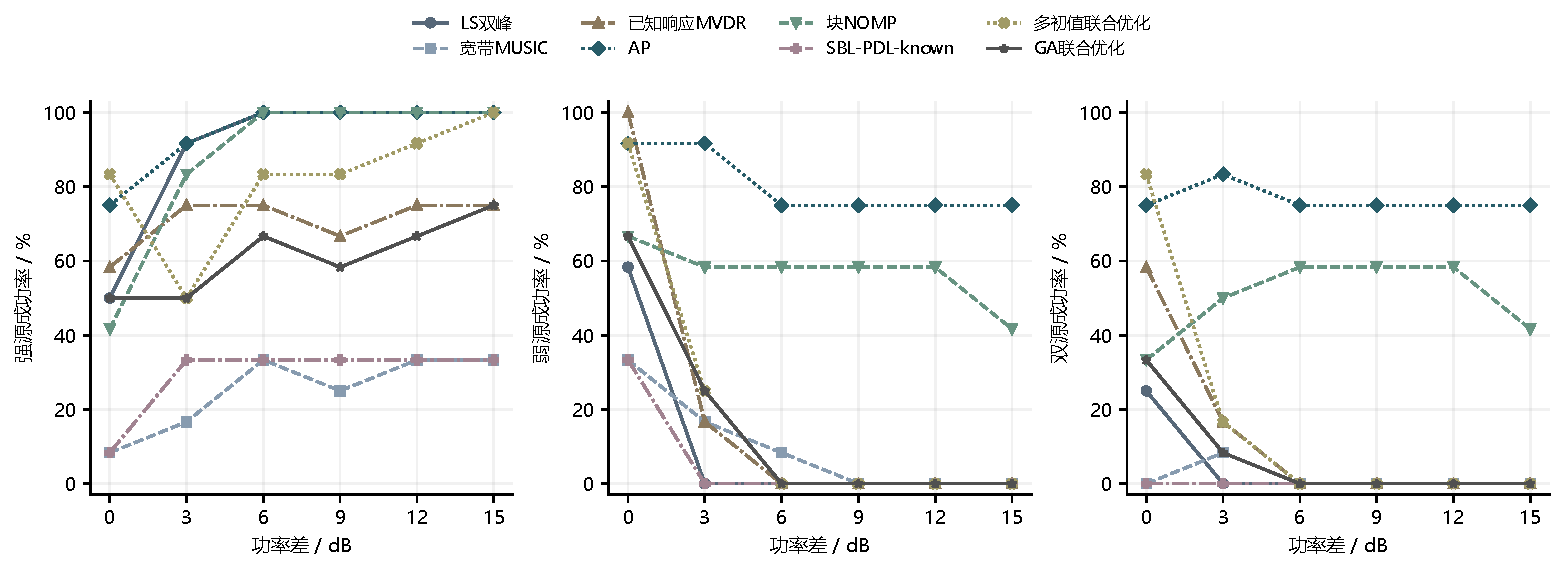
\includegraphics[width=\linewidth]{figures/g10_success.pdf}
\caption{60 s节点的强源、弱源及双源成功率。每档12个布局，成功阈值20 m。}\label{fig:g10-success}\end{figure}
表\ref{tab:g10-summary}和图\ref{fig:g10-success}显示，AP的弱源与双源成功数分别为58/72和55/72，弱源RMSE为17.80 m。其弱源成功数随功率差依次为11、11、9、9、9、9；在6--15 dB区间保持相同成功数。块NOMP对应为8、7、7、7、7、5，汇总弱源成功41/72。LS双峰、MUSIC、MVDR、SBL及两种通用联合优化在较大功率差下的弱源成功数明显下降。对这些数据，候选检测后充分利用联合拟合的逐源更新较为有效。

\begin{figure}[htbp]\centering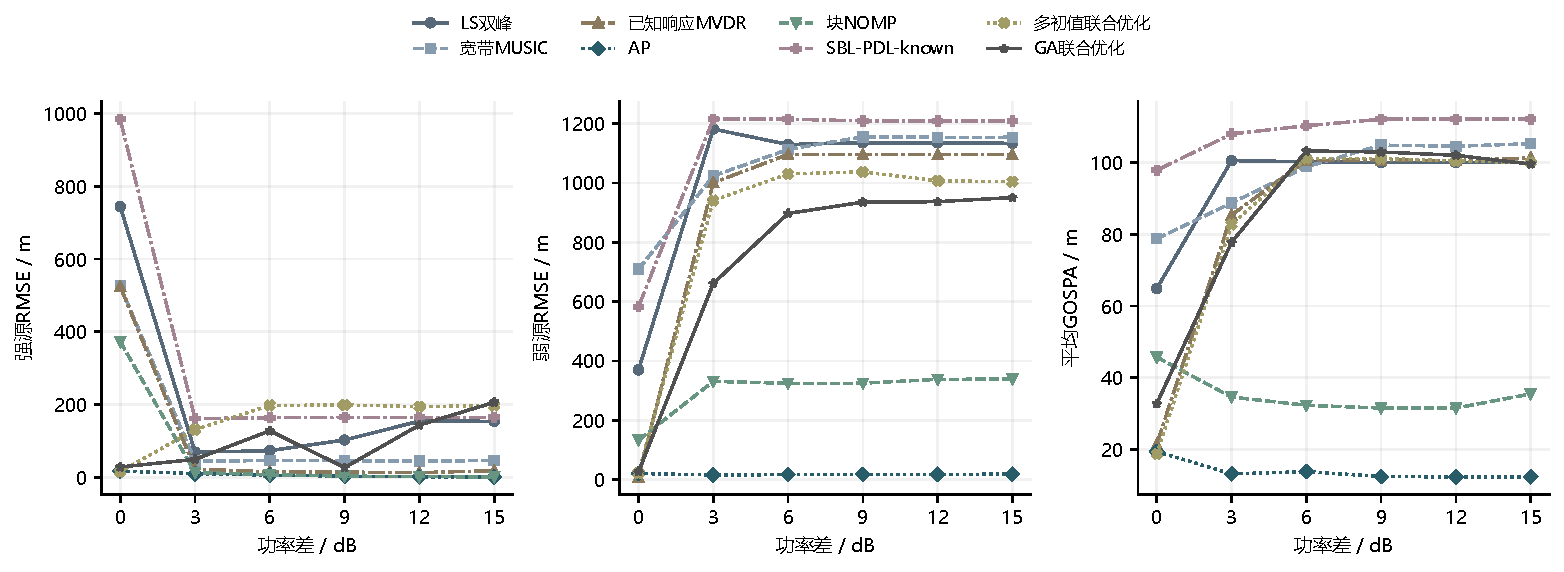
\includegraphics[width=\linewidth]{figures/g10_error.pdf}
\caption{强、弱源未截断RMSE及平均GOSPA随功率差的变化。}\label{fig:g10-error}\end{figure}
成功率与RMSE反映不同误差特征。块NOMP弱源成功率高于其余六种方法，但弱源RMSE为307.52 m，95\%误差分位约1027.47 m，仍有明显长尾。AP弱源95\%误差分位为45.12 m，最大误差为66.21 m。图\ref{fig:g10-cdf-strong}和图\ref{fig:g10-cdf-weak}展示六档功率差下的全部样本分布，避免仅用平均误差掩盖少量严重误定位。
\begin{figure}[htbp]\centering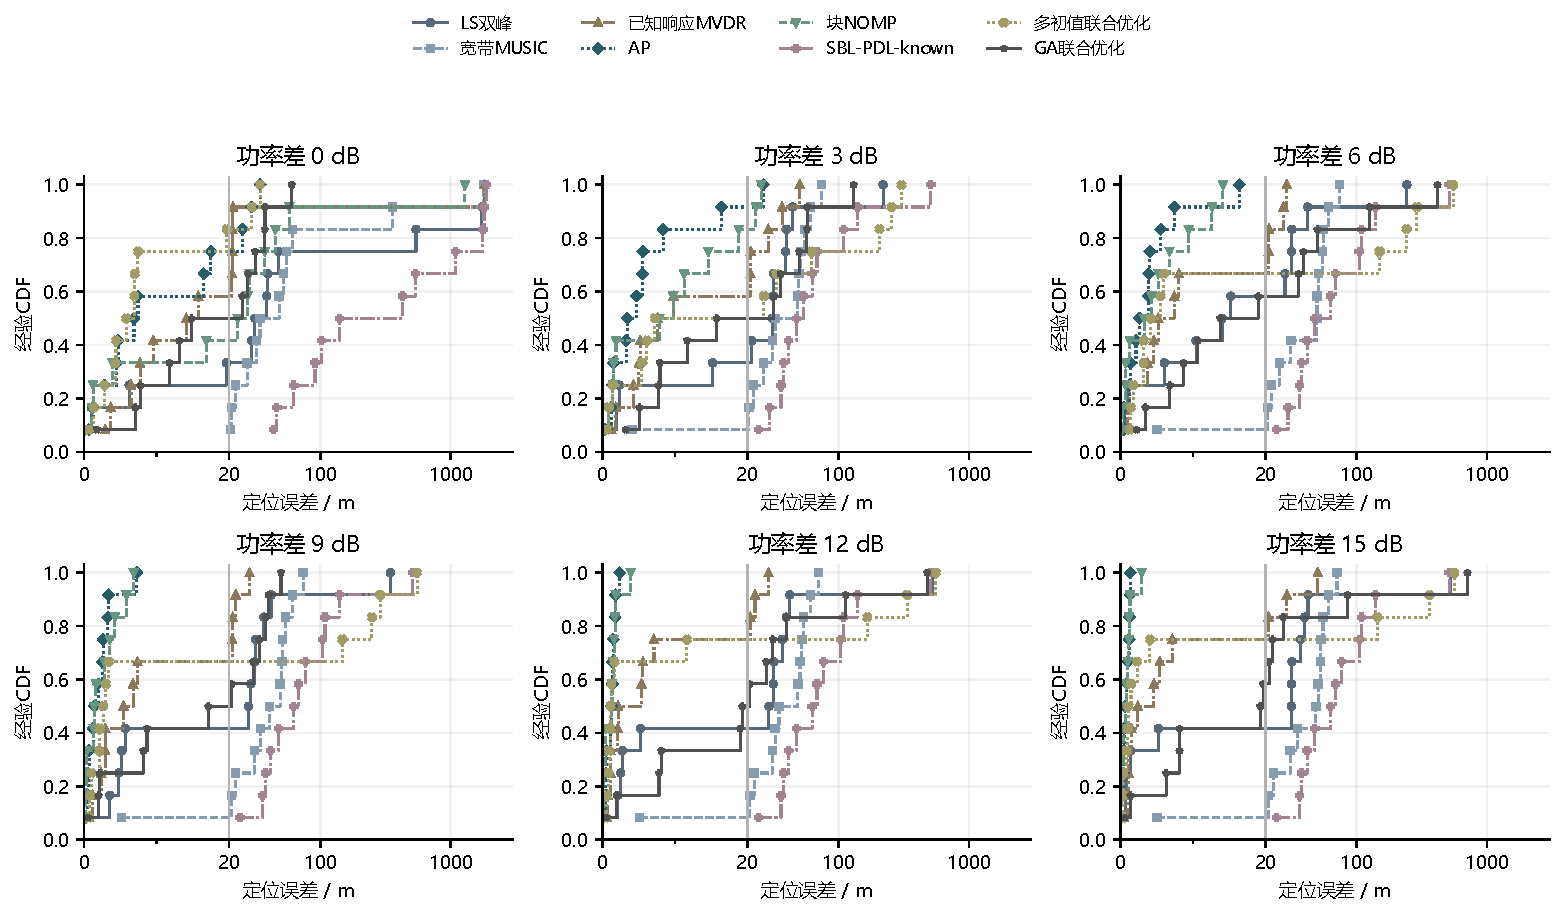
\includegraphics[width=\linewidth]{figures/g10_cdf_strong.pdf}
\caption{强源误差CDF。横轴在0--20 m线性显示，20 m以上采用对数尺度；每条曲线包含12条记录。}\label{fig:g10-cdf-strong}\end{figure}
\begin{figure}[htbp]\centering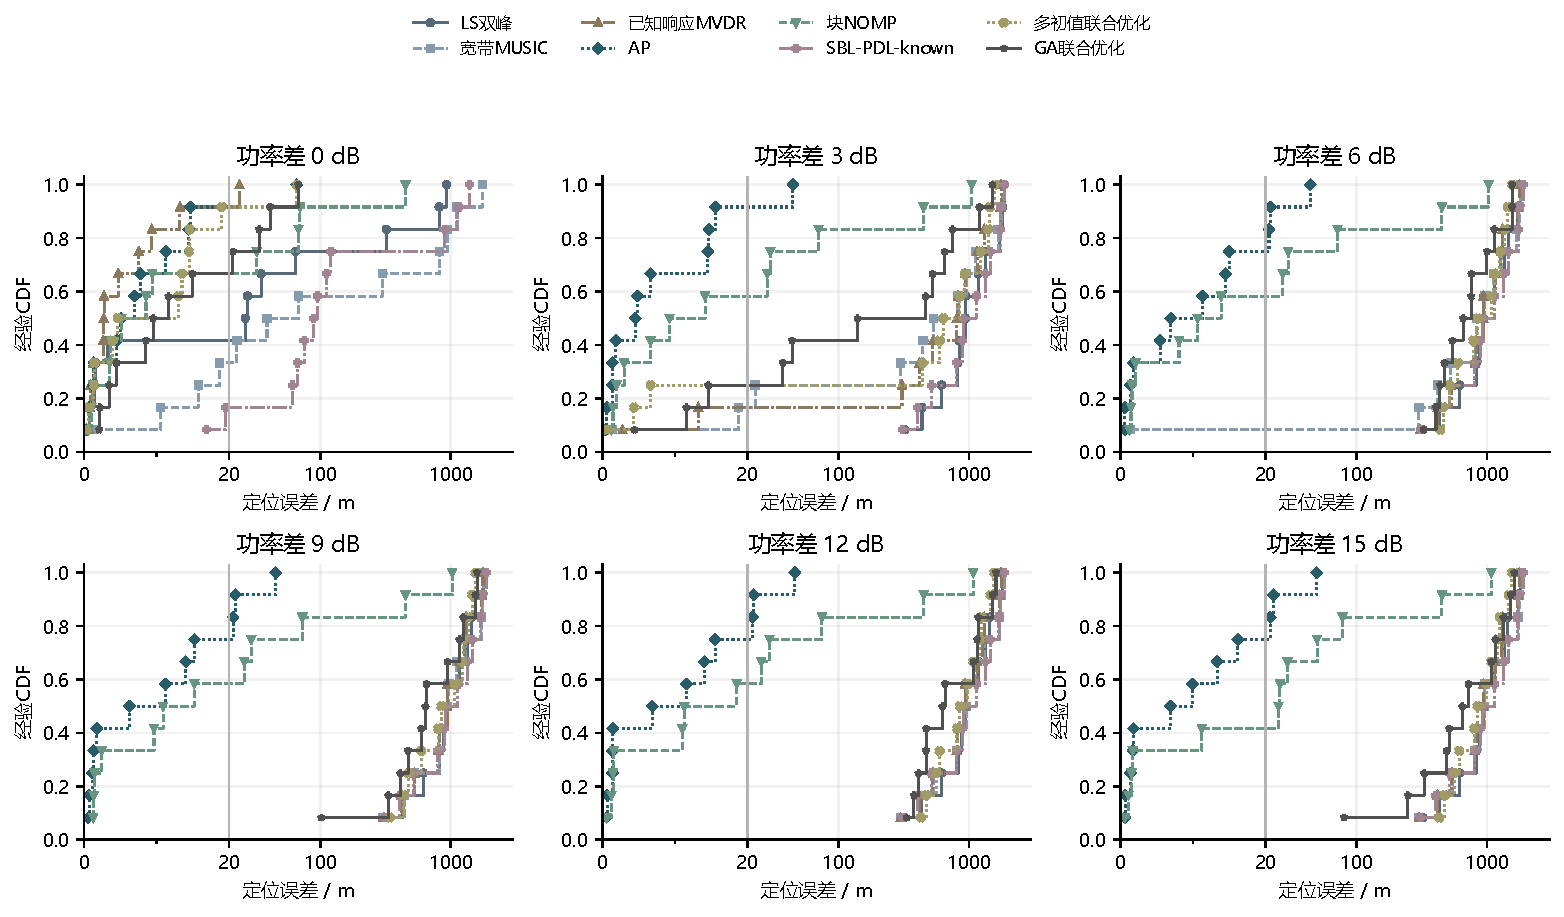
\includegraphics[width=\linewidth]{figures/g10_cdf_weak.pdf}
\caption{弱源误差CDF，坐标尺度与强源图一致。}\label{fig:g10-cdf-weak}\end{figure}

\subsection{早期估计、完整耗时与运算量}
\begin{figure}[htbp]\centering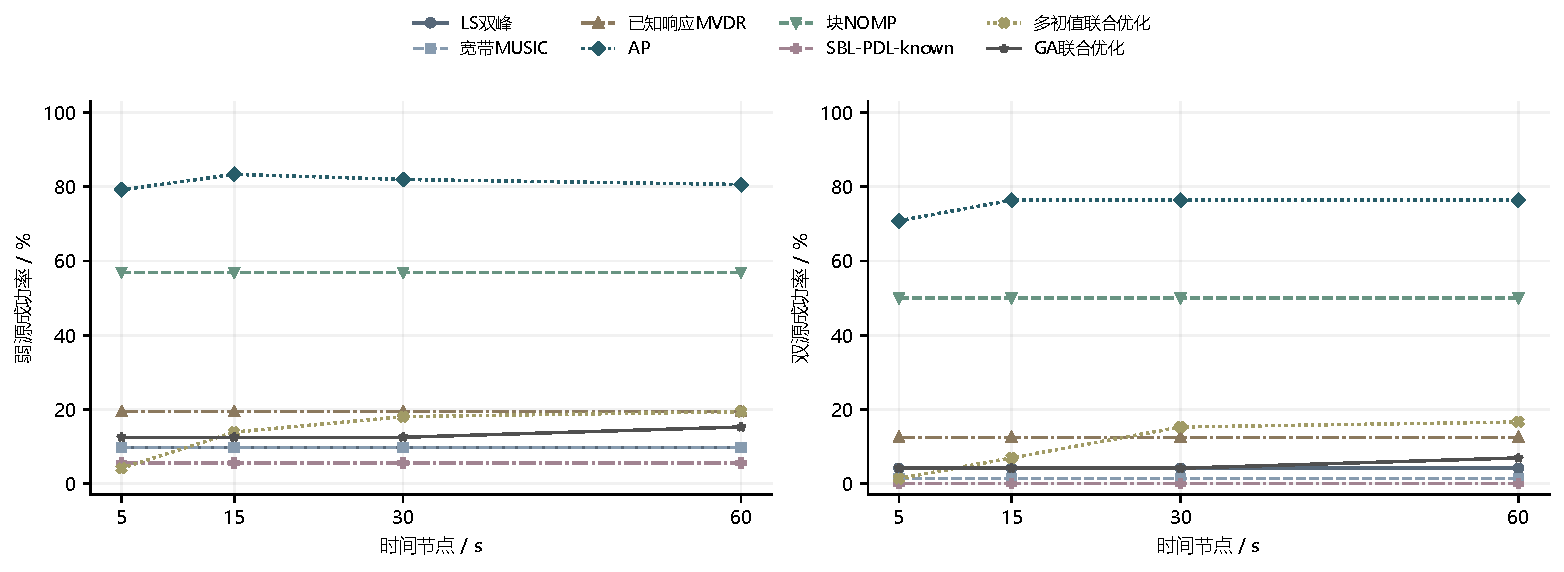
\includegraphics[width=\linewidth]{figures/g10_time.pdf}
\caption{共同时间节点下的定位成功率，每种方法包含72条混合记录。}\label{fig:g10-time}\end{figure}
AP在5 s节点已有57/72条弱源定位成功，15 s为60/72，30 s为59/72，60 s为58/72；对应双源成功数为51、55、55、55。AP保存联合残差更小的估计，但残差下降与真值误差下降并非逐样本一致。15 s以后强源RMSE继续下降，弱源成功数和RMSE则出现小幅变化。因此应分别考察获得较好估计的早期时间与完整搜索耗时。

\begin{figure}[htbp]\centering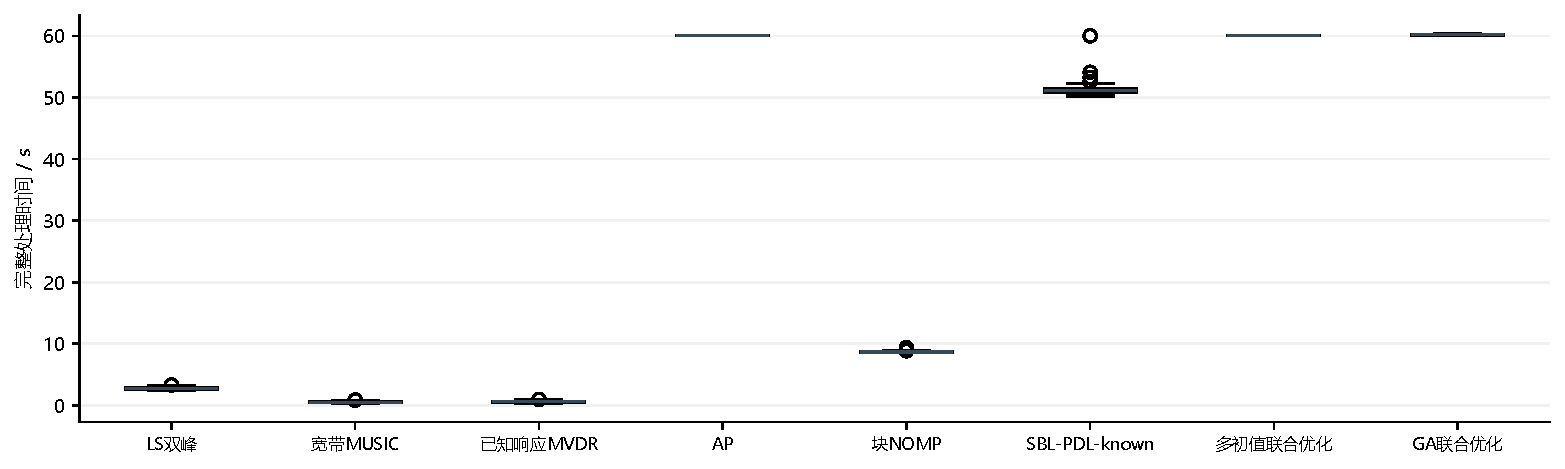
\includegraphics[width=\linewidth]{figures/g10_runtime.pdf}
\caption{72条混合记录的完整耗时分布。箱体为四分位范围，中线为中位数，须线采用1.5倍四分位距。}\label{fig:g10-runtime}\end{figure}
\begin{table}[htbp]\centering\small
\caption{混合源完整耗时与平均运算量}\label{tab:g10-cost}
\begin{tabular}{lrrrrr}\toprule
方法 & 中位数/s & 95\%分位/s & 响应点数/$10^9$ & 联合评价次数 & 协方差分解次数\\\midrule
LS双峰 & 2.71 & 3.05 & 0.677 & 0.0 & 0\\
宽带MUSIC & 0.53 & 0.76 & 0.044 & 0.0 & 4096\\
已知响应MVDR & 0.58 & 0.81 & 0.023 & 0.0 & 4096\\
AP & 60.05 & 60.10 & 1.187 & 532.9 & 0\\
块NOMP & 8.67 & 8.88 & 1.327 & 41.0 & 0\\
SBL-PDL-known & 51.17 & 52.40 & 2.785 & 0.0 & 1653646\\
多初值联合优化 & 60.06 & 60.10 & 0.185 & 542.9 & 0\\
GA联合优化 & 60.18 & 60.36 & 0.188 & 637.6 & 0\\
\bottomrule\end{tabular}
\end{table}
块NOMP平均完整耗时8.70 s，AP为60.06 s。前者较快结束，后者继续用剩余预算搜索和回访候选。表\ref{tab:g10-cost}同时给出响应计算点数、联合目标评价及协方差分解次数；不同方法的计算组织和每次评价内容不同，这些计数用于说明计算构成，实际代价以完整耗时为准。

\subsection{孤立源参照与困难布局}
\begin{figure}[htbp]\centering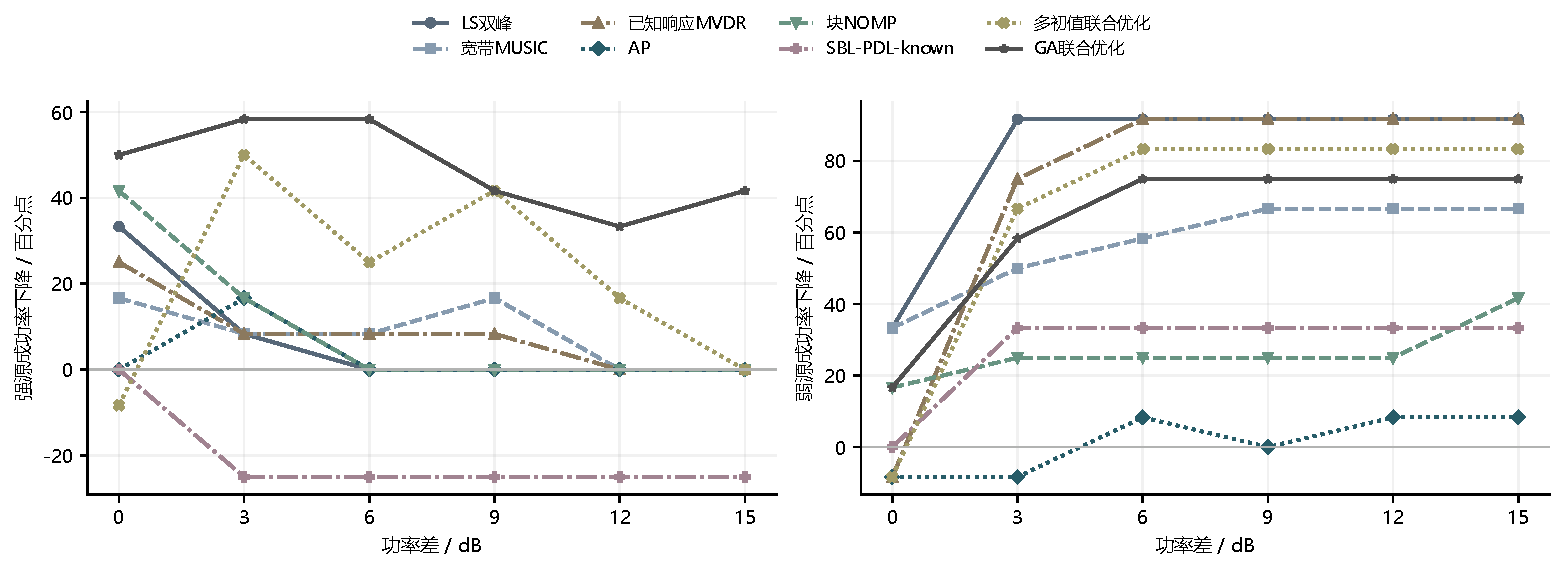
\includegraphics[width=\linewidth]{figures/g10_paired.pdf}
\caption{共同30 s节点下，孤立源成功率减去混合源成功率。正值表示加入另一源后成功率下降，每档均按12个布局配对。}\label{fig:g10-paired}\end{figure}
孤立弱源在LS、MUSIC、MVDR、AP、块NOMP、SBL、多初值和GA中的成功数依次为11、8、11、10、10、4、10、9（分母12）。在15 dB混合场景，相应弱源成功数为0、0、0、9、5、0、0、0。AP保留了大部分单源定位能力，块NOMP存在部分新增干扰损失。MUSIC和SBL的孤立强源成功数也分别为24/72和6/72，说明其本轮分段协方差与稀疏字典实现已有单源适配问题，混合表现需要结合这些参照理解。

AP在60 s节点的14次弱源失败集中于三个布局。以15 dB的30 s配对结果为例，这三个布局的孤立弱源误差约为2.75、21.60、26.32 m，混合弱源误差约为23.11、21.74、49.22 m。第一个布局新增阈值失败，第二个变化较小，第三个原已超过阈值且误差进一步增加。该配对关系区分了原有误差和强源加入后的损失，也提示后续应按布局研究耦合与搜索路径。

\subsection{代表性空间图}
图\ref{fig:g10-map0}--\ref{fig:g10-map15}使用预先选定的同一布局及同一组基础波形，分别展示0、9和15 dB。LS、MUSIC和MVDR为各自原生谱；SBL显示后验均值系数功率；AP、块NOMP、多初值与GA显示固定第一个估计位置后的条件LS切片。该切片反映另一候选位置的残差下降，并标明固定位置。

\begin{figure}[htbp]\centering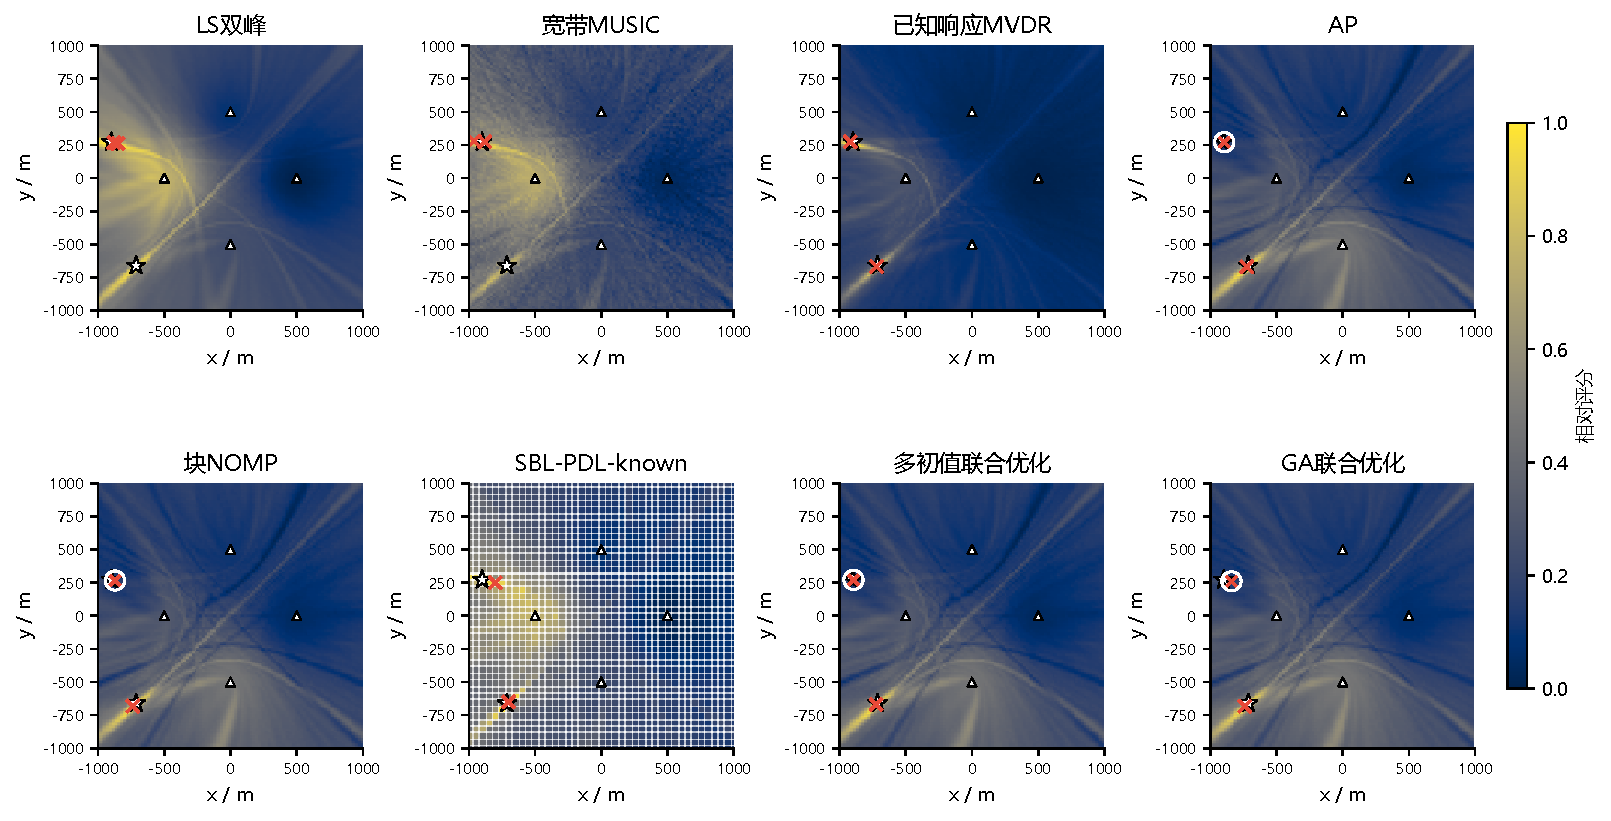
\includegraphics[width=\linewidth]{figures/g10_maps_0.pdf}
\caption{0 dB下八种方法的空间图。三角为站点，星号为真值，叉号为估计位置，空心圆为条件谱的固定位置。各面板按$(S-S_{\min})/(S_{\max}-S_{\min})$显示相对评分。}\label{fig:g10-map0}\end{figure}
\begin{figure}[htbp]\centering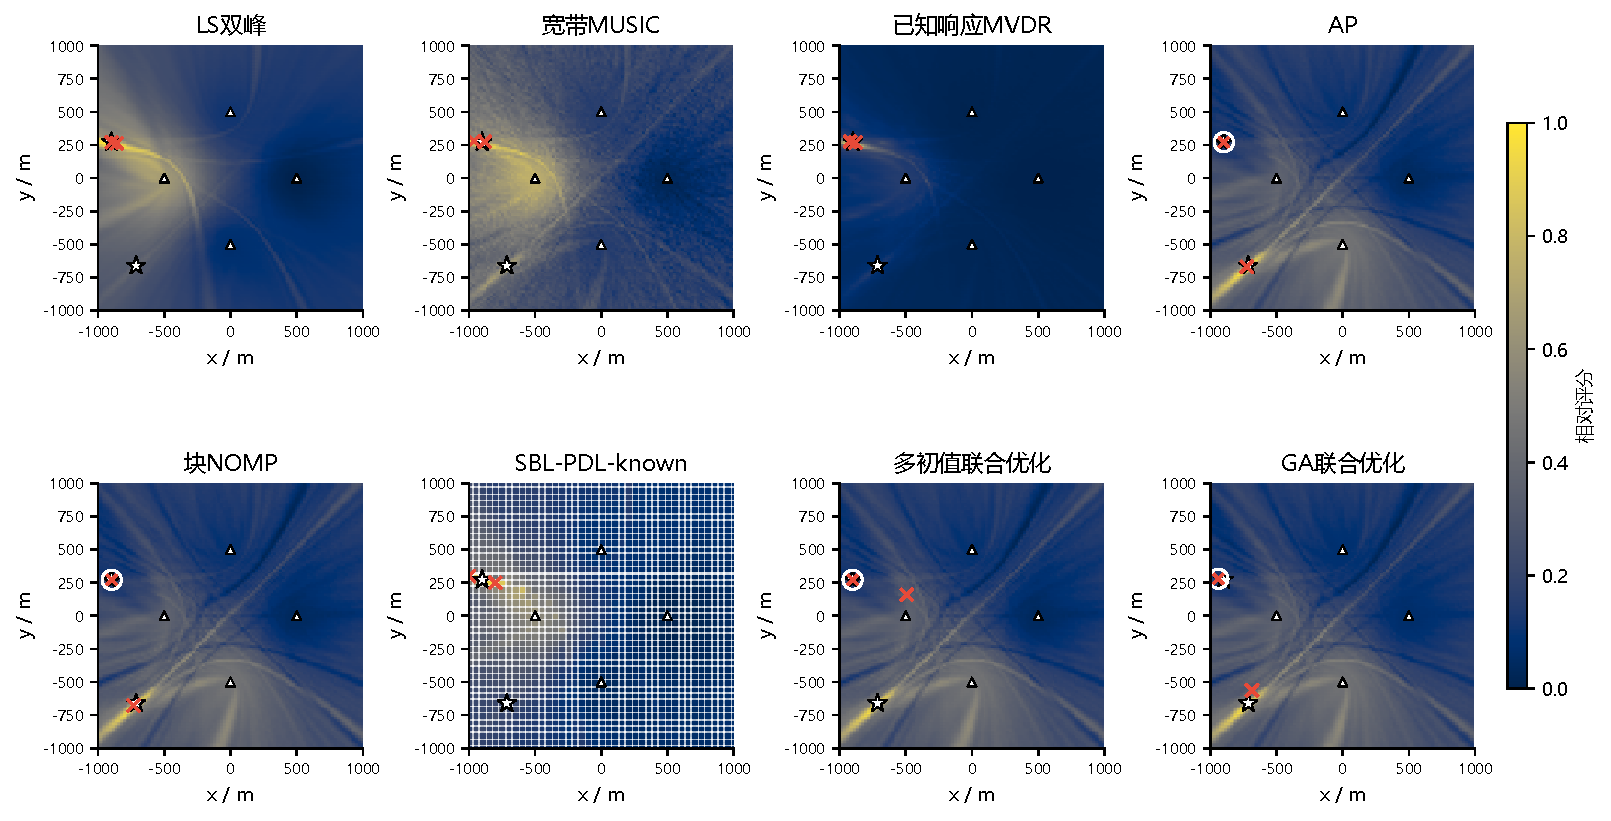
\includegraphics[width=\linewidth]{figures/g10_maps_9.pdf}
\caption{9 dB下的空间图。符号和归一化方式同图\ref{fig:g10-map0}。}\label{fig:g10-map9}\end{figure}
\begin{figure}[htbp]\centering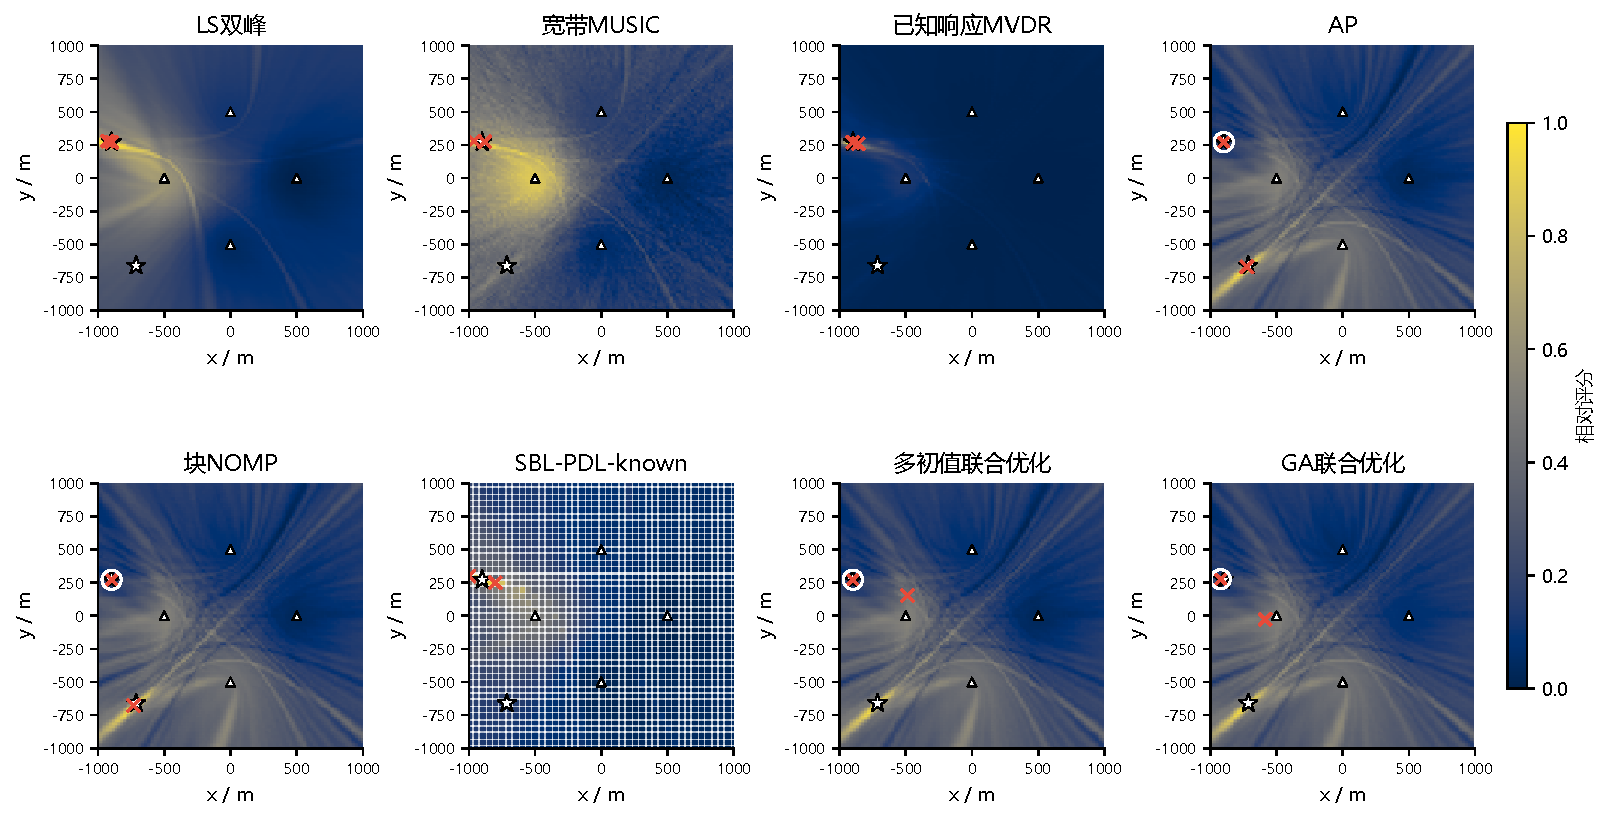
\includegraphics[width=\linewidth]{figures/g10_maps_15.pdf}
\caption{15 dB下的空间图。显示网格为20 m，SBL使用可局部移动的50 m字典点；估计标记来自连续位置输出。}\label{fig:g10-map15}\end{figure}
功率差增加后，单源扫描谱的显著峰更集中于强源附近。条件图则随已固定的估计位置变化；即使使用相同联合目标，不同搜索路径也可能得到不同切片。比较时同时观察真值附近的评分、最终估计和固定位置。空间图说明该代表性样本的定位过程，整体性能由前述12布局统计给出。

\section{讨论}\label{sec:new-discussion}
AP在较早时间节点获得了较高成功率，继续搜索主要改善联合拟合，弱源阈值成功数并未随之持续增加。后续可围绕候选排序、回访时机和停止条件分配计算，将早期有效搜索与后续收益较小的更新分开分析。

块NOMP以较少完整处理时间获得41/72的弱源成功数，但误差长尾仍较突出。AP与块NOMP在检测评分、循环更新和全局候选覆盖上不同；多初值与GA则从四维联合目标出发。下一步可在相同观测上追踪这些路径进入不同吸引域的过程，判断困难布局更需要候选覆盖还是联合位置调整。

MUSIC和SBL的单源参照偏低，首先需要检查短记录分段的子空间稳定性，以及字典间距、活动集选择和位置细化对单源估计的影响。当前结果已给出功率差增加时的退化现象，并显示AP和块NOMP具有不同的可靠性与耗时特点。是否提出新的定位方法，可在解决上述具体问题后进一步判断。


\FloatBarrier
\section{参考文献}\label{sec:5}
\begin{thebibliography}{99}
\small
\bibitem{ref01}C. H. Knapp and G. C. Carter, ``The generalized correlation method for estimation of time delay,'' \emph{IEEE Trans. Acoust., Speech, Signal Process.}, vol. 24, no. 4, pp. 321--327, 1976, doi: \href{https://doi.org/10.1109/TASSP.1976.1162830}{\nolinkurl{10.1109/TASSP.1976.1162830}}.

\bibitem{ref02}Y. T. Chan and K. C. Ho, ``A simple and efficient estimator for hyperbolic location,'' \emph{IEEE Trans. Signal Process.}, vol. 42, no. 8, pp. 1905--1915, 1994, doi: \href{https://doi.org/10.1109/78.301830}{\nolinkurl{10.1109/78.301830}}.

\bibitem{ref03}K. C. Ho, ``Bias reduction for an explicit solution of source localization using TDOA,'' \emph{IEEE Trans. Signal Process.}, vol. 60, no. 5, pp. 2101--2114, 2012, doi: \href{https://doi.org/10.1109/TSP.2012.2187283}{\nolinkurl{10.1109/TSP.2012.2187283}}.

\bibitem{ref04}A. J. Weiss and A. Amar, ``Direct position determination of multiple radio signals,'' \emph{EURASIP J. Appl. Signal Process.}, vol. 2005, no. 1, pp. 37--49, 2005, doi: \href{https://doi.org/10.1155/ASP.2005.37}{\nolinkurl{10.1155/ASP.2005.37}}.

\bibitem{ref05}J. C. Chen, R. E. Hudson, and K. Yao, ``Maximum-likelihood source localization and unknown sensor location estimation for wideband signals in the near-field,'' \emph{IEEE Trans. Signal Process.}, vol. 50, no. 8, pp. 1843--1854, 2002, doi: \href{https://doi.org/10.1109/TSP.2002.800420}{\nolinkurl{10.1109/TSP.2002.800420}}.

\bibitem{ref06}T. Tirer and A. J. Weiss, ``High resolution direct position determination of radio frequency sources,'' \emph{IEEE Signal Process. Lett.}, vol. 23, no. 2, pp. 192--196, 2016, doi: \href{https://doi.org/10.1109/LSP.2015.2503921}{\nolinkurl{10.1109/LSP.2015.2503921}}.

\bibitem{ref13} Z. Wang, D. Wang, F. Nie, and N. Zheng, ``TDOA-based direct position determination method with parametric dictionary learning,'' \emph{IEEE Sensors J.}, 2026, doi: \href{https://doi.org/10.1109/JSEN.2026.3693237}{\nolinkurl{10.1109/JSEN.2026.3693237}}.

\bibitem{ref07}W. Mantzel, J. Romberg, and K. G. Sabra, ``Round-robin multiple-source localization,'' \emph{J. Acoust. Soc. Am.}, vol. 135, no. 1, pp. 134--147, 2014, doi: \href{https://doi.org/10.1121/1.4835795}{\nolinkurl{10.1121/1.4835795}}.

\bibitem{ref08}B. Mamandipoor, D. Ramasamy, and U. Madhow, ``Newtonized orthogonal matching pursuit: Frequency estimation over the continuum,'' \emph{IEEE Trans. Signal Process.}, vol. 64, no. 19, pp. 5066--5081, 2016, doi: \href{https://doi.org/10.1109/TSP.2016.2580523}{\nolinkurl{10.1109/TSP.2016.2580523}}.

\bibitem{ref09}E. Tengan, T. Dietzen, F. Elvander, and T. van Waterschoot, ``Multi-source direction-of-arrival estimation using steered response power and group-sparse optimization,'' \emph{IEEE/ACM Trans. Audio, Speech, Lang. Process.}, vol. 32, pp. 3517--3531, 2024, doi: \href{https://doi.org/10.1109/TASLP.2024.3419417}{\nolinkurl{10.1109/TASLP.2024.3419417}}.

\bibitem{ref15}J. Capon, ``High-resolution frequency-wavenumber spectrum analysis,'' \emph{Proc. IEEE}, vol. 57, no. 8, pp. 1408--1418, 1969, doi: \href{https://doi.org/10.1109/PROC.1969.7278}{\nolinkurl{10.1109/PROC.1969.7278}}.

\bibitem{ref16}K. Deb and R. B. Agrawal, ``Simulated binary crossover for continuous search space,'' \emph{Complex Syst.}, vol. 9, no. 2, pp. 115--148, 1995. [Online]. Available: \url{https://www.complex-systems.com/abstracts/v09_i02_a02/}.

\bibitem{ref10}D. Zachariah and P. Stoica, ``Cramér--Rao bound analog of Bayes rule,'' \emph{IEEE Signal Process. Mag.}, vol. 32, no. 2, pp. 164--168, 2015, doi: \href{https://doi.org/10.1109/MSP.2014.2365593}{\nolinkurl{10.1109/MSP.2014.2365593}}.

\bibitem{ref12}A. S. Rahmathullah, Á. F. García-Fernández, and L. Svensson, ``Generalized optimal sub-pattern assignment metric,'' in \emph{Proc. 20th Int. Conf. Inf. Fusion (FUSION)}, Xi'an, China, 2017, pp. 1--8, doi: \href{https://doi.org/10.23919/ICIF.2017.8009645}{\nolinkurl{10.23919/ICIF.2017.8009645}}.

\bibitem{ref11}E. Weinstein and A. J. Weiss, ``Fundamental limitations in passive time-delay estimation---Part II: Wide-band systems,'' \emph{IEEE Trans. Acoust., Speech, Signal Process.}, vol. 32, no. 5, pp. 1064--1078, 1984, doi: \href{https://doi.org/10.1109/TASSP.1984.1164429}{\nolinkurl{10.1109/TASSP.1984.1164429}}.
\end{thebibliography}

\clearpage
\appendix
\section{已知相对增益模型及求解}\label{sec:2}

本附录保留原有搜索策略及条件评分的补充分析。传播相对响应与正文一致，以下使用未归一化响应$\mathbf A_m$及其源系数表示。基本LS关系见正文第\ref{sec:current-model}节；原有A--D策略及附录\ref{sec:3}的实验独立保留。

% Source block 21
\subsection{场景、符号与假设}\label{sec:2.1}

% Source block 22
考虑$L$个已知位置的同步接收站和$K$个静止源，本文仿真取$L=4$、$K=2$。站位置为$\mathbf{r}_\ell\in\mathbb{R}^2$，源位置为$\mathbf{p}_k\in\mathbb{R}^2$，待估位置向量为
% Source block 23
\begin{equation}\label{eq:2.1}
\theta = [\mathbf{p}_1^{T},\ldots,\mathbf{p}_K^{T}]^{T} \in\mathbb{R}^{2K}.
\end{equation}

% Source block 24
假设信号经直达路径传播，各站噪声为相互独立的白色圆对称复高斯噪声。源波形、发射功率和公共初相均未知，并包含在源信号中。仿真与集中最小二乘方法采用相同的$1/d$衰减和基带时延相位，不设逐站幅相偏差。图\ref{fig:2.1}给出一个双源场景，仿真参数见表\ref{tab:3.1}。

% Source block 25
\begin{figure}[H]
\centering
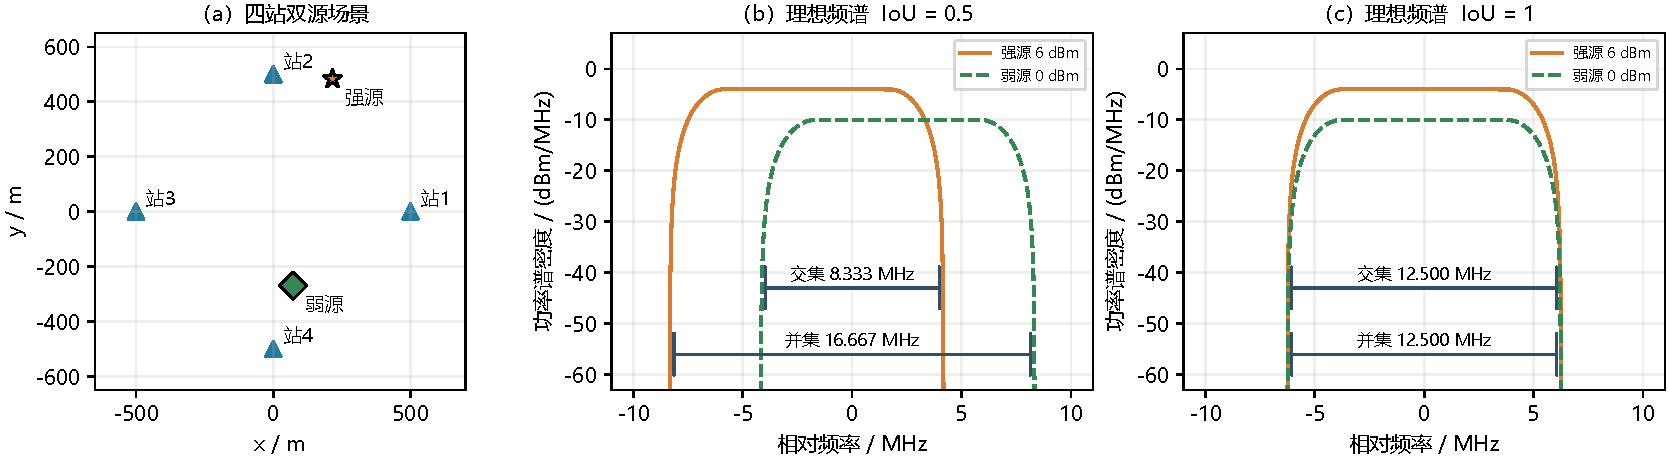
\includegraphics[width=\linewidth]{figures/fig_2_1.pdf}
\caption{四站单天线场景与两类频谱重叠。}\label{fig:2.1}
\begin{minipage}{\linewidth}\small
（a）四站位于半径500 m的圆周上；强、弱源位置分别为 $(215.85,483.29)$ m 和 $(72.77,-270.30)$ m，取自仿真中的一个双源场景。（b）、（c）符号率10 MHz、滚降系数0.25的理想根升余弦（RRC）成形信号功率谱，单源支持宽度均为12.5 MHz。图示功率为6 dBm和0 dBm，仅用于表现6 dB强弱差；纵轴为功率谱密度 dBm/MHz。IoU按频率支持的交集宽度除以并集宽度定义，而非按曲线重叠面积定义：中心频率间隔为 $12.5/3$ MHz时，交集与并集分别为 $25/3$ 和 $50/3$ MHz，IoU恰为0.5；中心重合时IoU为1。仿真的位置范围及功率定义见表\ref{tab:3.1}。
\end{minipage}
\end{figure}

% Source block 28
\begin{table}[H]
\centering
\caption{主要符号与维度。}\label{tab:2.1}
\small
\setlength{\tabcolsep}{4pt}
\renewcommand{\arraystretch}{1.2}
\begin{tabularx}{\linewidth}{Y{0.85}Y{1.35}Y{0.8}}
\toprule
\textbf{符号} & \textbf{含义} & \textbf{维度或单位} \\
\midrule
$\mathbf{r}_\ell,\mathbf{p}_k$ & 站位置、源位置 & $2\times1$，m \\
$d_{\ell k},\tau_{\ell k}$ & 传播距离、传播时延 & m，s \\
$F_s,T_s,T$ & 采样率、采样间隔、观测时长 & Hz，s，s \\
$\mathbf{x}_m,\mathbf{s}_m$ & 第 $m$ 个频点的站观测、源系数 & $L\times1$、$K\times1$ \\
$\mathbf{A}_m$ & 位置参数化的响应矩阵 & $L\times K$ \\
$\Pi_m^\perp$ & 响应列空间的正交补投影 & $L\times L$ \\
$\mathbf{D}_m$ & 均值对实位置参数的导数 & $L\times2K$ \\
$\mathbf{J}_{\theta}^{\mathrm{eff}}$ & 消去未知波形后的位置信息 & $2K\times2K$，m$^{-2}$ \\
\bottomrule
\end{tabularx}
\end{table}

% Source block 30
上标$T$、$H$和$\dagger$分别表示转置、共轭转置和Moore–Penrose伪逆；$\|\cdot\|$表示欧氏范数。

% Source block 31
\subsection{接收信号模型}\label{sec:2.2}

% Source block 32
参照宽带联合定位模型\cite{ref05}，设连续复基带源信号为$s_k(t)$，传播距离、时延和幅度衰减为
% Source block 33
\begin{equation}\label{eq:2.2}
d_{\ell k}=\|\mathbf{p}_k-\mathbf{r}_\ell\|, \qquad \tau_{\ell k}=\frac{d_{\ell k}}{c}, \qquad g_{\ell k}=\frac{1}{d_{\ell k}}.
\end{equation}

% Source block 34
衰减的公共比例常数并入$s_k(t)$。每站记录$N$个采样点，观测模型为
% Source block 35
\begin{equation}\label{eq:2.3}
x_\ell[n] =\sum_{k=1}^{K}g_{\ell k} s_k(nT_s-\tau_{\ell k})+w_\ell[n], \quad n=0,\ldots,N-1, \qquad w_\ell[n]\sim\mathcal{CN}(0,\sigma_t^2).
\end{equation}

% Source block 36
其中$T_s=1/F_s$，观测时长为$T=NT_s$，$c$为传播速度。复噪声满足$\mathbb{E}|w_\ell[n]|^2=\sigma_t^2$，实部和虚部方差均为$\sigma_t^2/2$。仿真中的两源采用独立二进制相移键控（BPSK）数据、符号时序及初相，经RRC脉冲成形产生；定位算法不使用比特或逐源频谱真值。源的统计独立性不意味着有限记录的交叉项恰为零。

% Source block 37
采用除以$N$的DFT约定，
% Source block 38
\begin{equation}\label{eq:2.4}
X_{\ell m} =\frac{1}{N}\sum_{n=0}^{N-1}x_\ell[n]e^{-j2\pi mn/N}, \qquad \sigma_f^2=\frac{\sigma_t^2}{N}.
\end{equation}

% Source block 39
正负频率均保留，$f_m$为带符号基带频率。采用忽略观测窗边缘效应的频域近似模型\cite{ref04,ref05}，将各站的同一频点观测叠成向量，得到
% Source block 40
\begin{equation}\label{eq:2.5}
\mathbf{x}_m =\mathbf{A}_m(\theta)\mathbf{s}_m +\mathbf{n}_m, \qquad \mathbf{n}_m\sim\mathcal{CN}(\mathbf{0},\sigma_f^2\mathbf{I}_L),
\end{equation}
% Source block 41
\begin{equation}\label{eq:2.6}
[\mathbf{a}_m(\mathbf{p}_k)]_\ell =\frac{e^{-j2\pi f_m d_{\ell k}/c}}{d_{\ell k}}, \qquad \mathbf{A}_m=[\mathbf{a}_m(\mathbf{p}_1),\ldots,\mathbf{a}_m(\mathbf{p}_K)].
\end{equation}

% Source block 42
本文载频相位约定为$f_c=0$，下文的似然推导与信息分析均基于式（\ref{eq:2.5}）所采用的频域模型。

% Source block 43
每个频点的源系数$\mathbf{s}_m$独立拟合，位置在所有频点之间共享。响应列缩放由源系数吸收，与正文的单位范数响应表示等价。

\subsection{波形消元的对应关系}\label{sec:2.3}
正文式\eqref{eq:2.8}--\eqref{eq:2.7}已给出波形消元与集中LS目标。将单位列响应$\mathbf Q_m$换为未归一化响应$\mathbf A_m$，相应系数按列尺度调整，集中目标保持不变。下文记$\Pi_m^\perp=\mathbf I-\mathbf A_m\mathbf A_m^\dagger$，用于条件评分和搜索界的推导。

% Source block 54
\subsection{逐源搜索与联合更新}\label{sec:2.4}

% Source block 55
直接枚举$K$个二维位置组合的计算量随源数迅速增加。本文采用逐源初始化与交替位置更新，并周期性重新搜索已估源的位置。更新一个位置时，先固定其他位置，其响应记为$\mathbf{B}_m$，并定义
% Source block 56
\begin{equation}\label{eq:2.11}
\begin{aligned}
&\Pi_{B,m}^\perp =\mathbf{I}-\mathbf{B}_m\mathbf{B}_m^\dagger, \\
& \mathbf{r}_m=\Pi_{B,m}^\perp\mathbf{x}_m, \quad \mathbf{u}_m(\mathbf{p})=\Pi_{B,m}^\perp\mathbf{a}_m(\mathbf{p}).
\end{aligned}
\end{equation}

% Source block 57
新增源的系数和原有源系数均允许重新拟合。线性LS消元后，新增位置带来的残差下降量为
% Source block 58
\begin{equation}\label{eq:2.12}
Q(\mathbf{p}\mid\mathbf{B}) = \sum_m \frac{|\mathbf{a}_m(\mathbf{p})^H\Pi_{B,m}^\perp\mathbf{x}_m|^2} {\mathbf{a}_m(\mathbf{p})^H\Pi_{B,m}^\perp\mathbf{a}_m(\mathbf{p})}.
\end{equation}

% Source block 59
分母为投影后候选响应的能量，因此该式与联合LS的增量一致。投影及候选响应归一化也见于Round-robin多源定位\cite{ref07}。当$\mathbf{u}_m=\mathbf{0}$时，新增响应没有增加列空间，该频点的增量定义为零；其余情况下有
% Source block 60
\begin{equation}\label{eq:2.13}
0\leq \frac{|\mathbf{u}_m^H\mathbf{r}_m|^2}{\|\mathbf{u}_m\|^2} \leq\|\mathbf{r}_m\|^2.
\end{equation}

% Source block 61
实现中以尺度检查处理退化频点，并用观测总能量$E_x=\sum_m\|\mathbf{x}_m\|^2$归一化评分。同一记录内这一归一化不改变候选排序。

表\ref{tab:methods}定义本文比较的完整定位方法。普通DPD直接选取空间谱峰；A、B、C、D采用集中最小二乘目标，其主要差别在候选搜索。表中的AP表示交替投影（alternating projection）求解。

\begin{table}[H]
\centering
\caption{定位方法与候选搜索策略。}\label{tab:methods}
\small
\setlength{\tabcolsep}{4pt}
\renewcommand{\arraystretch}{1.2}
\begin{tabularx}{\linewidth}{Y{0.85}Y{1.05}Y{1.1}}
\toprule
\textbf{方法} & \textbf{候选搜索} & \textbf{目标函数与位置更新} \\
\midrule
普通DPD & 时延补偿相关矩阵的最大特征值评分、粗细搜索 & 双峰选取与分别精修，不作逐源投影 \\
A：多初值AP & 粗网格、多初值 & 集中LS、L-BFGS-B、交替更新及循环搜索 \\
B：普通区域搜索 & 按当前得分细分区域，保留全局探索 & 与A相同 \\
C：响应变化引导搜索 & 在B中加入响应变化量排序 & 与A相同 \\
D：补充全局搜索 & 完整B后逐源5 m扫描及前5个候选精修 & 同一集中LS目标，再作2轮局部交替更新 \\
\bottomrule
\end{tabularx}
\end{table}

普通DPD以站间能量归一化后的时延补偿相关矩阵最大特征值评分，经粗细选峰与分别精修输出位置。其与A、B、C的比较反映完整求解流程的差异。

A、B、C使用相同的普通DPD初始候选搜索，耗时计入总时间。共同配置为5个初值、最多5轮交替更新、每次局部优化最多30次迭代，第3、5轮重新搜索已估源。B、C每次最多细分48个区域，每4次保留1次全局探索；C的响应变化量定义见第\ref{sec:2.5.3}节，排序权重固定为0.25。

原始混合观测先经逐站RMS归一化产生最大特征值谱候选，随后A--C在原始观测的集中LS目标下执行多初值、逐源搜索、连续精修及全部波形重估。搜索不限于初始位置邻域，第3、5轮还有重新搜索；D进一步补充全区域扫描。初始化可能影响有限预算下的结果，但现有比较未单独量化这一影响。

% Source block 62
\begin{figure}[!htbp]
\centering
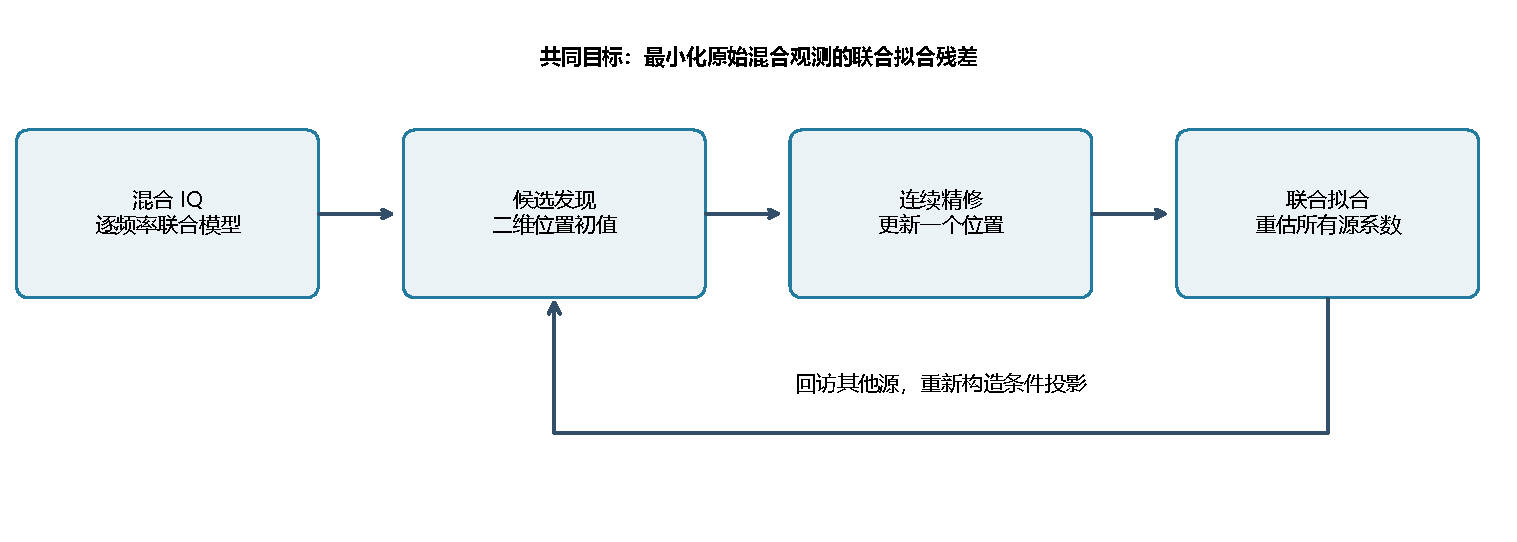
\includegraphics[width=\linewidth]{figures/fig_2_2.pdf}
\caption{共同联合求解流程。}\label{fig:2.2}
\begin{minipage}{\linewidth}\small
候选搜索提供初值，连续优化更新位置，所有源的频率系数重新拟合；回访时重新计算条件投影。A、B、C、D使用同一集中最小二乘目标，候选覆盖范围和计算量不同。
\end{minipage}
\end{figure}

% Source block 65
每次接受位置更新后，重新拟合所有源系数，再更新其他位置。保留新旧解中联合残差较小者，可保证残差不增加，但不能保证进入真实位置附近的吸引域。

为考察候选覆盖不足的影响，方法D在完整方法B的输出上增加一轮全局位置更新：依次固定另一个源，在全区域5 m网格上计算式（\ref{eq:2.12}），保留前5个候选并连续精修；两个位置均更新后，再作两轮局部交替更新。每一步均保留联合残差较小的解。该过程只使用观测和当前估计，真实位置仅用于结果评价。

% Source block 66
\subsection{当前的理论与算法难点}\label{sec:2.5}

% Source block 67
\subsubsection{局部可辨识性与全局搜索}\label{sec:2.5.1}

% Source block 68
若$K\geq L$且响应矩阵满行秩，逐频自由系数可拟合任意观测，集中目标退化。本文$L=4,K=2$时，满列秩响应每频点保留两个复残余维度，但位置能否在局部辨识仍取决于响应导数。

% Source block 69
令$\mathbf{D}_m=\partial(\mathbf{A}_m\mathbf{s}_m)/\partial\theta^T$，求导时保持源系数固定。在响应局部满列秩、噪声协方差已知且与参数无关的条件下，消去未知复波形的等效位置信息为\cite{ref05,ref10}
% Source block 70
等效信息的表达式见正文式\eqref{eq:new-information}，其中可等价使用本附录的$\mathbf D_m$和$\Pi_m^\perp$。

% Source block 71
当该矩阵正定时，其逆给出正则、局部无偏位置估计的Cramér--Rao下界（CRLB）。该界描述真实位置附近的精度，不说明求解器能否进入这一邻域。远处局部极值和阈值效应还需另行分析\cite{ref11}。

% Source block 72
\subsubsection{投影损失与强源位置误差}\label{sec:2.5.2}

% Source block 73
设单频点的强、弱源响应分别为$\mathbf{a}_s$和$\mathbf{a}_w$。固定真实强源响应，令$\Pi_s^\perp=\mathbf{I}-\mathbf{a}_s\mathbf{a}_s^H/\|\mathbf{a}_s\|^2$，则响应相关系数与弱源能量保留比例为
% Source block 74
\begin{equation}\label{eq:2.15}
\rho =\frac{\mathbf{a}_s^H\mathbf{a}_w}{\|\mathbf{a}_s\|\|\mathbf{a}_w\|}, \qquad \eta =\frac{\|\Pi_s^\perp\mathbf{a}_w\|^2}{\|\mathbf{a}_w\|^2} =1-|\rho|^2.
\end{equation}

% Source block 75
响应相似时，消去强源也会移除部分弱源能量。宽带保留比例需按各频点的实际弱源能量加权，不能用一个频点代表全部观测。固定投影下的噪声协方差为$\sigma_f^2\Pi_s^\perp$，在投影保留子空间的正交基中仍可作同方差LS处理。

% Source block 76
若强源位置估计误差为$\delta\mathbf{p}_s$，记$\mathbf{H}_{s,m}=\partial\mathbf{a}_m(\mathbf{p}_s)/\partial\mathbf{p}_s^T$，$s_{sm}$为该源在第$m$个频点的系数。在小误差条件下，残留强源能量的主导项为
% Source block 77
\begin{equation}\label{eq:2.16}
E_{\mathrm{leak}} \approx \sum_m |s_{sm}|^2 \|\Pi_{s,m}^\perp\mathbf{H}_{s,m}\delta\mathbf{p}_s\|^2.
\end{equation}

% Source block 78
残留随强源功率和误差方向变化。因此，满足定位成功判据的强源估计，仍可能干扰弱源评分。由于投影位置通常由同一观测估计，其误差与残余之间存在统计依赖。

% Source block 79
\subsubsection{窄峰采样与候选保留}\label{sec:2.5.3}

% Source block 80
式（\ref{eq:2.13}）保证增量评分有界，但当投影响应范数较小时，其归一化方向仍可能随位置迅速变化。固定其他位置，设二维位置偏移为$\delta$；在光滑局部极大点$\mathbf{p}_\star$附近，令$\mathbf{H}_\star=-\nabla^2Q(\mathbf{p}_\star)\succ0$，有
% Source block 81
\begin{equation}\label{eq:2.17}
Q(\mathbf{p}_\star+\delta) =Q(\mathbf{p}_\star) -\frac12\delta^T\mathbf{H}_\star\delta +O(\|\delta\|^3).
\end{equation}

% Source block 82
二维正方网格间隔为$h$时，最近格点满足$\|\delta\|^2\leq h^2/2$。在局部展开有效的范围内，
% Source block 83
\begin{equation}\label{eq:2.18}
Q(\mathbf{p}_\star)-Q(\mathbf{p}_{\mathrm{grid}}) \leq\frac{\lambda_{\max}(\mathbf{H}_\star)h^2}{4}+O(h^3).
\end{equation}

% Source block 84
即使真实位置附近存在高峰，邻近格点也可能因采样损失排在远处候选之后。统一缩小网格间隔能减少此类损失，但二维评分点数随$h^{-2}$增长。需要在有限计算量下判断哪些区域值得继续搜索。

% Source block 85
本文比较的一种区域选择规则使用投影响应的空间变化量。设参与评分的频点数为$M$，$\partial_i$表示对位置坐标$p_i$求导。固定其他位置，定义
% Source block 86
\begin{equation}\label{eq:2.19}
\zeta(\mathbf{p}) =\frac{1}{M}\sum_{m=1}^{M}\sum_{i\in\{x,y\}} \left[ \frac{\|\partial_i\mathbf{u}_m\|^2}{\|\mathbf{u}_m\|^2} - \frac{|\mathbf{u}_m^H\partial_i\mathbf{u}_m|^2}{\|\mathbf{u}_m\|^4} \right].
\end{equation}

% Source block 87
该量扣除纯整体幅相变化后，衡量响应方向的局部敏感性。方法C将其乘以区域半宽的平方，转为排名后与评分排名加权组合。它未直接使用残余观测，因而响应变化快不一定意味着该区域包含高评分候选。其作用需通过同预算实验检验。

\subsubsection{区域评分上界与候选排除}\label{sec:region-bound}

为判断未充分采样的区域是否仍可能包含更高分位置，考虑固定其他源时的条件评分上界。设正方形区域$\mathcal C$的中心为$\mathbf p_c$、半边长为$h$，区域内任一点到中心的距离不超过$\Delta_{\mathcal C}=\sqrt{2}h$。数值搜索以$d_0=1$ m截断站点附近的距离，避免$1/d$奇异；区域界采用同一响应。记$d_\ell^c=\max(\|\mathbf p_c-\mathbf r_\ell\|,d_0)$、$d_{\ell,-}=\max(d_\ell^c-\Delta_{\mathcal C},d_0)$。由距离变化界和复指数相位差界，单站响应变化不超过
\begin{equation}\label{eq:response-bound}
\begin{aligned}
\varepsilon_{\ell m}
&=\frac{\Delta_{\mathcal C}}{d_\ell^c d_{\ell,-}}
+\frac{2}{d_\ell^c}\sin\!\left[\frac12\min\!\left(\pi,\frac{2\pi|f_m|\Delta_{\mathcal C}}{c}\right)\right],\\
\varepsilon_m&=\left(\sum_{\ell=1}^{L}\varepsilon_{\ell m}^2\right)^{1/2}.
\end{aligned}
\end{equation}

正交投影不增加向量范数，因此$\|\mathbf u_m(\mathbf p)-\mathbf u_m(\mathbf p_c)\|\leq\varepsilon_m$。以下以$\mathbf u_m^c=\mathbf u_m(\mathbf p_c)$简记中心响应，并定义
\begin{equation}\label{eq:cone-parameters}
t_m=\min\!\left(1,\frac{\varepsilon_m}{\|\mathbf u_m^c\|}\right),\qquad
v_m=\frac{|(\mathbf u_m^c)^H\mathbf r_m|}{\|\mathbf u_m^c\|\,\|\mathbf r_m\|}.
\end{equation}

当$t_m<1$时，响应方向的偏转角不超过$\arcsin t_m$。据此限制候选响应与残余的夹角，得到归一化评分的区域上界
\begin{equation}\label{eq:cell-upper}
\begin{aligned}
\frac{Q(\mathbf p\mid\mathbf B)}{E_x}&\leq U(\mathcal C)
=\frac{1}{E_x}\sum_m\|\mathbf r_m\|^2 H(v_m,t_m),\quad \mathbf p\in\mathcal C,\\
H(v,t)&=\begin{cases}
\bigl(v\sqrt{1-t^2}+t\sqrt{1-v^2}\bigr)^2,&t<\sqrt{1-v^2},\\
1,&t\geq\sqrt{1-v^2}.
\end{cases}
\end{aligned}
\end{equation}

残余为零时，该频点贡献为零；中心投影响应退化时，取该频点的残余能量作为上界。若$U(\mathcal C)$低于已找到的最佳评分，即可排除该区域；否则可优先细分上界较高的区域。上界是否足够紧、其计算代价是否低于直接补点评分，需要由实验判断。第\ref{sec:3.10}节将其与得分优先细分、均匀及错位网格搜索比较。

% Source block 88
本文要解决的问题是：在给定观测和计算预算下，发现可能被粗搜索遗漏的弱源候选，并通过联合位置更新减轻强源估计误差的影响。

% Source block 90
\section{已知相对增益条件下的实验结果}\label{sec:3}

本附录完整保留既有实验。原比较组、新布局比较组与固定诊断组分别统计，分母、成功判据和处理时间沿用原记录。原信号采用随机共同中心频率，包含6/12 dB功率差、3 dB弱源带内SNR及不同记录长度和频谱重叠条件；正文采用零中心完全重叠、6 dB弱源带内SNR及六档功率差，两组结果分别解释。

% Source block 91
\subsection{仿真设置}\label{sec:3.1}

% Source block 92
本章先在32个独立布局上比较方法A、B、C，并分析其失败记录；随后在六个新布局上比较完整方法B与D。区域上界的比较则使用固定24条诊断记录，仅更新弱源位置。三类结果分别统计。第\ref{sec:3.7}节另给出投影机理的频域数值示例。

% Source block 93
\begin{table}[!htbp]
\centering
\caption{主要仿真参数与第一组方法比较设置。}\label{tab:3.1}
\small
\setlength{\tabcolsep}{4pt}
\renewcommand{\arraystretch}{1.2}
\begin{tabularx}{\linewidth}{Y{0.65}Y{1.35}}
\toprule
\textbf{项目} & \textbf{设置} \\
\midrule
接收几何 & 四站：约 $(500,0),(0,500),(-500,0),(0,-500)$ m \\
空间范围 & $[-1000,1000]^2$ m²，连续源位置 \\
源数与间距 & 已知 $K=2$；源间距至少 300 m，源站距离至少 150 m \\
波形 & 两个独立 BPSK／RRC 源，符号率 10 MHz，滚降系数 0.25 \\
采样与长度 & $F_s=100$ MHz；$N=4096,16384$ \\
标称带宽与重叠 & 12.5 MHz；频谱支持 IoU 为 0.5、1 \\
弱源功率 & 全网平均带内信噪比（SNR）为3 dB \\
强弱差 & 全网平均接收功率差为 6、12 dB \\
独立布局与实现 & 32 个布局，每布局 2 组波形／噪声实现 \\
混合条件数 & $32\times2\times2\times2\times2=512$ 条 \\
单源对照 & 每种长度各 128 条孤立弱源、128 条孤立强源 \\
主预算 $T_0$ & 4096 点为 3.7216 s；16384 点为 11.5376 s \\
预算曲线 & $0.5T_0,T_0,2T_0$，取截止时已经完成的输出 \\
\bottomrule
\end{tabularx}
\end{table}

% Source block 95
短、长记录使用同一连续波形与噪声流的前缀。比较两档功率差时，弱信号和噪声逐样本保持不变，只改变强源幅度。独立性以布局为单位，置信区间采用按布局成组的配对重采样。

% Source block 96
方法参数在各组比较前固定。第一组的失败诊断用于选择补充搜索配置；方法D的5 m网格、候选数和更新轮数在六个新布局的结果计算前固定。孤立／混合对照保持弱信号及噪声不变，用于分析加入强源后的额外损失。

方法D的比较使用完整执行的B作为基线，不沿用第一组的预算截止输出。B、D采用相同的分块双精度评分实现；D的完整耗时包含B及后续补充搜索。计算平台为NVIDIA RTX 4070 Ti SUPER，PyTorch 2.8.0，CPU线程数为4。

% Source block 100
\subsection{评价指标}\label{sec:3.2}

% Source block 101
令真实集合与输出集合分别为 $\mathcal{P}$ 和 $\widehat{\mathcal{P}}$。在半径 $r$ 内，成功评价先最大化可匹配源数，再以平方距离及固定规则打破平局。令$I_{w,j}(r)$和$I_{s,j}(r)$分别表示第$j$条记录中弱、强源是否按此规则成功匹配的指示量，弱源成功率和双源同时成功率为
% Source block 102
\begin{equation}\label{eq:3.1}
\begin{aligned}
&R_w(r)=\frac{1}{n_{\mathrm{rec}}}\sum_{j=1}^{n_{\mathrm{rec}}}I_{w,j}(r), \\
& R_{\mathrm{both}}(r) =\frac{1}{n_{\mathrm{rec}}}\sum_{j=1}^{n_{\mathrm{rec}}}I_{s,j}(r)I_{w,j}(r).
\end{aligned}
\end{equation}

% Source block 103
其中 $n_{\mathrm{rec}}$ 为记录数。成功半径取最大站间基线的2\%，即$r=0.02\max_{\ell,q}\|\mathbf{r}_\ell-\mathbf{r}_q\|=20$ m。均方根误差（RMSE）、95\%分位数（P95）和误差累积分布函数（CDF）另用平方距离最优匹配，保留全部匹配误差。两种匹配分别用于成功判断和距离误差统计。

% Source block 104
集合误差采用广义最优子模式分配（GOSPA）距离\cite{ref12}，参数为$p=2,\alpha=2,\kappa=100$ m。其部分匹配形式为
% Source block 105
\begin{equation}\label{eq:3.2}
d_{\mathrm G}^2(\mathcal{P},\widehat{\mathcal{P}}) = \min_{\gamma} \left[ \sum_{(i,j)\in\gamma}\|\mathbf{p}_i-\widehat{\mathbf{p}}_j\|^2 +\frac{\kappa^2}{2}(K+\widehat K-2|\gamma|) \right],
\end{equation}

% Source block 106
其中 $\gamma$ 为一对一部分匹配，$\kappa$是GOSPA的截断参数，与20 m成功半径分别定义。表中的GOSPA是逐记录$d_{\mathrm G}$的平均值；RMSE是未截断平方距离误差均值的平方根。

% Source block 107
完整在线时间包含共同候选前端、物理评分、投影、搜索与连续精修。三档预算快照来自同一次运行轨迹，统计时仍使用原布局分组。

% Source block 108
\subsection{孤立弱源与混合弱源}\label{sec:3.3}

% Source block 109
\begin{figure}[!htbp]
\centering
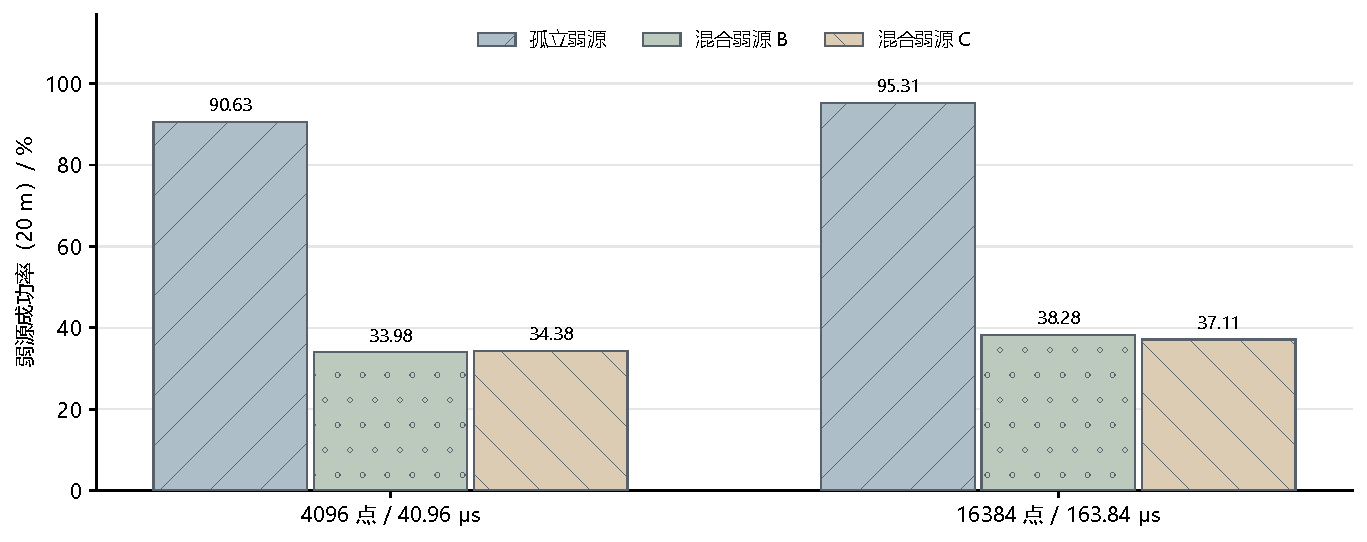
\includegraphics[width=\linewidth]{figures/fig_3_1.pdf}
\caption{同一弱信号与噪声条件下的孤立／混合对照。}\label{fig:3.1}
\begin{minipage}{\linewidth}\small
每种长度包含128条孤立弱源及256条混合条件；混合条件的两档功率差共享对应弱信号。混合结果取主预算$T_0$，评价半径20 m。
\end{minipage}
\end{figure}

% Source block 112
\begin{table}[!htbp]
\centering
\caption{孤立弱源与混合弱源成功数。}\label{tab:3.3}
\small
\setlength{\tabcolsep}{4pt}
\renewcommand{\arraystretch}{1.2}
\begin{tabularx}{\linewidth}{Y{0.6}Y{1.4}Y{1}Y{1}}
\toprule
\textbf{长度} & \textbf{孤立弱源，共同参照} & \textbf{B混合弱源} & \textbf{C混合弱源} \\
\midrule
4096点 & 116/128（90.625\%） & 87/256（33.984\%） & 88/256（34.375\%） \\
16384点 & 122/128（95.313\%） & 98/256（38.281\%） & 95/256（37.109\%） \\
\bottomrule
\end{tabularx}
\end{table}

% Source block 114
两种长度下，孤立弱源的成功率分别为90.63\%和95.31\%，加入强源后，方法B、C降至约34\%—38\%。对照保持弱信号和噪声不变，反映了强源叠加后的额外损失。记录长度由4096增加至16384点时，混合弱源成功率有所提高，但与孤立弱源之间仍有较大差距。

% Source block 115
站间强弱关系由几何及发射功率共同形成。当前按全网平均接收功率定义强弱，不要求同一源在每站都占优。因此还需结合实际响应分析源间竞争，而不能仅由一个全局功率比预测成败。

% Source block 116
\subsection{逐源处理与候选排序}\label{sec:3.4}

% Source block 117
\begin{figure}[!htbp]
\centering
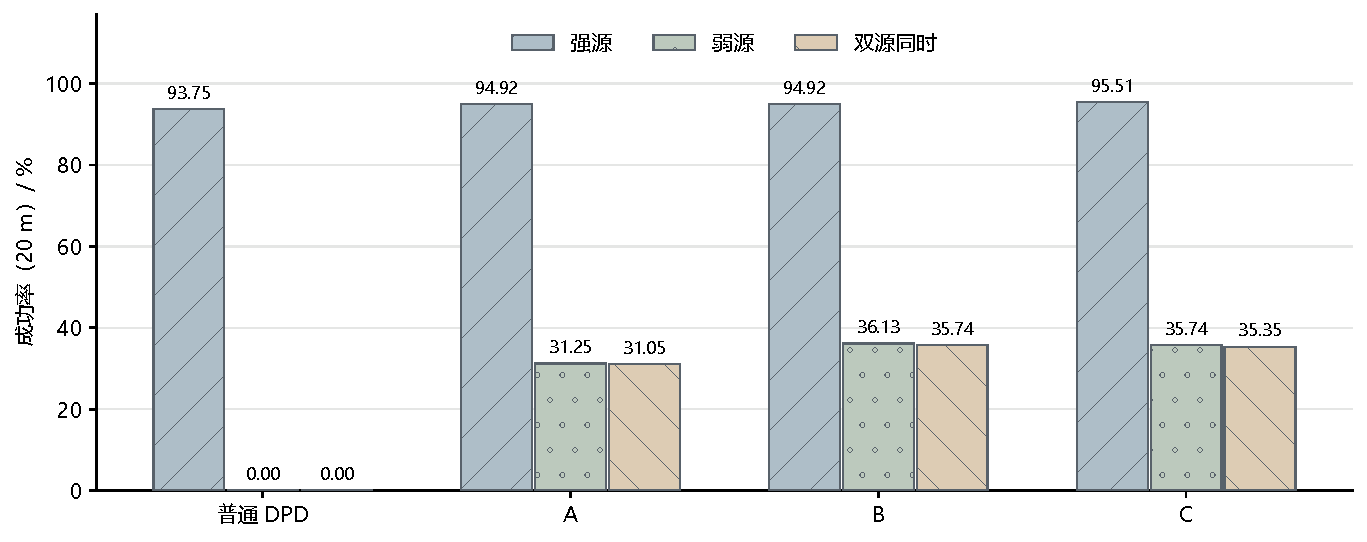
\includegraphics[width=\linewidth]{figures/fig_3_2.pdf}
\caption{主预算下的完整方法比较。}\label{fig:3.2}
\begin{minipage}{\linewidth}\small
合并两种长度，每方法512条混合条件，评价半径20 m。A、B、C采用共同的逐源投影和联合更新；方法D在另一组新布局上单独比较，见第\ref{sec:3.9}节。
\end{minipage}
\end{figure}

% Source block 120
\begin{table}[!htbp]
\centering
\caption{主预算 $T_0$ 下的总体结果。}\label{tab:3.4}
\small
\setlength{\tabcolsep}{4pt}
\renewcommand{\arraystretch}{1.2}
\begin{tabularx}{\linewidth}{Y{0.95}Y{1.05}Y{1.15}Y{1.05}Y{1.1}Y{0.85}Y{0.85}}
\toprule
\textbf{方法} & \textbf{弱源成功率} & \textbf{双源同时成功率} & \textbf{强源成功率} & \textbf{平均GOSPA / m} & \textbf{RMSE / m} & \textbf{P95 / m} \\
\midrule
普通DPD & 0.00\% & 0.00\% & 93.75\% & 101.73 & 807.21 & 1684.03 \\
A & 31.25\% & 31.05\% & 94.92\% & 64.16 & 259.85 & 616.25 \\
B & 36.13\% & 35.74\% & 94.92\% & 60.46 & 256.71 & 612.58 \\
C & 35.74\% & 35.35\% & 95.51\% & 61.36 & 242.01 & 579.53 \\
\bottomrule
\end{tabularx}
\end{table}

% Source block 122
普通DPD大多能够定位强源，但弱源未满足20 m成功判据。A、B、C采用逐源投影和联合更新后，弱源成功率提高至31.25\%—36.13\%。C相对A提高4.49个百分点，按32个布局配对重采样得到的95\%区间为$[0.59,8.79]$个百分点；相对B则降低0.39个百分点，区间为$[-5.27,3.91]$个百分点。

% Source block 123
逐例比较中，C恢复了B的22条弱源失败记录，同时使B原先成功的24条记录失败，净减少2条成功。C的RMSE较低，但GOSPA与20 m成功率未同步改善。因此，新增响应变化量排序相对普通区域搜索B尚未显示稳定收益。

% Source block 124

% Source block 125
\subsection{条件评分与失败原因}\label{sec:3.5}

% Source block 126
对方法B的512条混合记录作条件评分分析，固定其主预算输出。在327条弱源失败中，分别比较原强源估计下的真实弱源与返回点评分、固定真实强源后的两点评分，以及真实位置对与返回位置对的联合目标。真实位置仅用于诊断，不参与候选生成。

% Source block 127
\begin{table}[!htbp]
\centering
\caption{全部失败记录的条件评分分析。}\label{tab:3.5}
\small
\setlength{\tabcolsep}{4pt}
\renewcommand{\arraystretch}{1.2}
\begin{tabularx}{\linewidth}{Y{0.65}Y{0.8}Y{1.15}Y{1.2}Y{1.2}}
\toprule
\textbf{记录长度} & \textbf{B弱源失败数} & \textbf{原强源估计下真弱源评分更高} & \textbf{真实强源位置下真弱源评分更高} & \textbf{真实位置对的联合拟合更好} \\
\midrule
4096点 & 169 & 147 & 159 & 158 \\
16384点 & 158 & 145 & 155 & 155 \\
合计 & 327 & 292 & 314 & 313 \\
\bottomrule
\end{tabularx}
\end{table}

% Source block 129
292/327条，即89.30\%的失败，在保持原强源估计与评分函数不变时，真实弱源位置的评分已高于返回点。以真实弱源位置为初值作局部精修，得到评分更高且误差不超过20 m的局部解的记录共295条；两项统计允许重叠。这些比较表明，大部分失败记录存在求解器未找到的更优位置。

% Source block 130
在原强源估计下真弱源评分不占优的35条记录中，22条在替换为真实强源位置后获得评分优势，其中1条原强源误差已小于20 m。这说明定位成功半径并不能直接作为强源精修的停止条件，弱源评分仍可能受到强源位置误差影响。

% Source block 131
327条失败中，313条的真实位置对具有更小的联合拟合残差。其余记录不能仅凭真实位置处的评分归因于搜索遗漏，还需区分局部估计偏差与错误吸引域。以下加密搜索对照用于进一步检验候选覆盖的作用。

% Source block 132
\begin{figure}[!htbp]
\centering
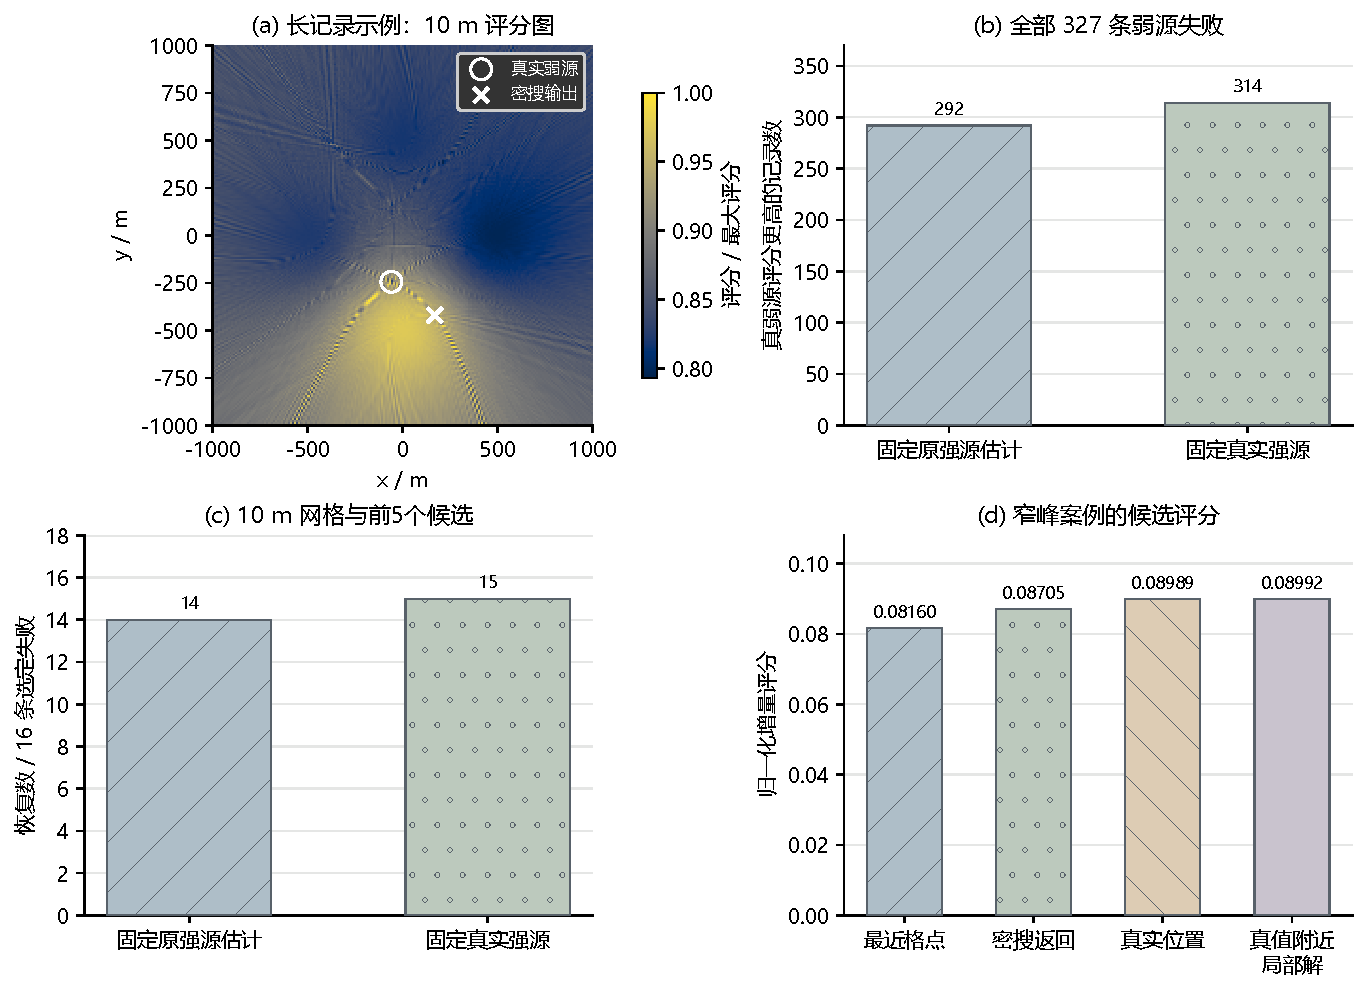
\includegraphics[width=.92\linewidth]{figures/fig_3_3.pdf}
\caption{从评分地形到搜索归因。}\label{fig:3.3}
\begin{minipage}{\linewidth}\small
（a）辅助长记录示例：IoU=0.5、$N=65536$，全区域10 m评分图，标出真实弱源与密搜输出；该例不计入两种主记录长度的统计。（b）方法B全部327条弱源失败的条件评分。（c）预先选定的16条失败记录中，加密搜索在20 m判据下的恢复数；另8条历史对照在更新后均达到20 m。（d）窄峰案例：$N=4096$、IoU=1、功率差12 dB，固定真实强源，比较四类位置的评分。
\end{minipage}
\end{figure}

% Source block 135
\subsection{加密搜索与窄峰遗漏}\label{sec:3.6}

% Source block 136
搜索诊断使用此前按100 m判据选定的24条记录，不从当前327条失败中重新抽样。样本按长度、重叠和功率差分成8组，每组包含2条历史失败和1条历史对照，共涉及4个布局。16条历史失败的初始误差均超过20 m；8条对照中，初始只有6条满足20 m，另2条误差为61.42 m和63.37 m。以下保留这两个固定分组，并统一按20 m评价更新结果。诊断固定强源位置，以全区域10 m扫描、前5个候选及连续精修重求弱源。

% Source block 137
\begin{table}[!htbp]
\centering
\caption{固定样本的搜索诊断。}\label{tab:3.6}
\small
\setlength{\tabcolsep}{4pt}
\renewcommand{\arraystretch}{1.2}
\begin{tabularx}{\linewidth}{Y{1}Y{0.6}Y{1.15}Y{1.1}Y{1.15}}
\toprule
\textbf{条件} & \textbf{记录数} & \textbf{固定原强源后密搜成功} & \textbf{固定真实强源后密搜成功} & \textbf{真实位置对初始化后双源成功} \\
\midrule
历史失败组 & 16 & 14 & 15 & 16 \\
历史对照组 & 8 & 8 & 8 & 8 \\
\bottomrule
\end{tabularx}
\end{table}

% Source block 139
保持原强源位置不变，加密搜索使16条选定失败中的14条定位成功。这表明这些记录可通过改变搜索恢复，但目的抽样的恢复比例不能作为全部失败记录的成功率估计。

% Source block 140
两个剩余案例揭示了不同原因。在4096点、IoU=1、功率差6 dB的耦合案例中，原强源误差为558.73 m；固定该位置时，弱源密搜误差仍为1095.56 m；改用真实强源位置后降至0.828 m。这是强源位置耦合的具体实例。

% Source block 141
在4096点、IoU=1、功率差12 dB的窄峰案例中，强源误差仅0.073 m，10 m密搜仍返回约125.48 m的弱源误差。固定真实强源位置时，其评分关系如下。

% Source block 142
\begin{table}[!htbp]
\centering
\caption{一个窄峰遗漏案例的评分。}\label{tab:3.7}
\small
\setlength{\tabcolsep}{4pt}
\renewcommand{\arraystretch}{1.2}
\begin{tabularx}{\linewidth}{Y{1.1}Y{1}Y{0.9}}
\toprule
\textbf{位置} & \textbf{归一化增量评分} & \textbf{与真实弱源的距离} \\
\midrule
最近10 m格点 & 0.08159913 & 4.523 m \\
密搜返回位置 & 0.08704823 & 125.36 m \\
真实弱源位置 & 0.08989170 & 0 m \\
真值附近局部解 & 0.08992482 & 0.803 m \\
\bottomrule
\end{tabularx}
\end{table}

% Source block 144
最近格点与真实位置仅相距4.523 m，评分却低于远处返回点。该例中，从正确区域启动局部精修可达到亚米级误差，但10 m网格加Top5没有保留相应候选。这一现象与式（\ref{eq:2.17}）—（\ref{eq:2.18}）描述的采样损失及排名变化相符。

% Source block 145
在同一组24条记录上，进一步比较网格间隔与候选保留数。固定原强源估计，采用同一分块评分实现时，10 m网格与前5个候选恢复14/16条历史失败；将候选数增至32仍恢复14条，而5 m网格与前5个候选恢复15条。三种配置均使8条历史对照达到20 m，包括初始未达标的2条记录。对应16条失败的单次弱源补充搜索平均耗时分别为2.95、3.61和11.29 s，不包含此前求得强源位置的耗时。这表明，对该组样本，扩大候选数不能替代更细的空间采样。

辅助长记录诊断在另16个选定条件中，固定评分、改变搜索使20 m弱源恢复数从3增至8。该组仅用于说明相似的候选遗漏现象，不与本章主样本合并统计。

% Source block 146
\subsection{强源位置偏差的投影数值示例}\label{sec:3.7}

% Source block 147
为说明小位置误差如何产生强源残留，采用式（\ref{eq:2.6}）的频域响应，计算投影后的能量。四站坐标与图\ref{fig:2.1}相同，强、弱源分别位于$(650,-300)$ m和$(-800,-700)$ m。65个频点均匀覆盖$[-6.25,6.25]$ MHz，复噪声方差取1，每频点全网平均SNR分别为15、3 dB；固定随机相位的源谱作为未知确定性系数处理。该例用于说明投影机理，不参与BPSK定位成功率统计。

% Source block 148
\begin{figure}[!htbp]
\centering
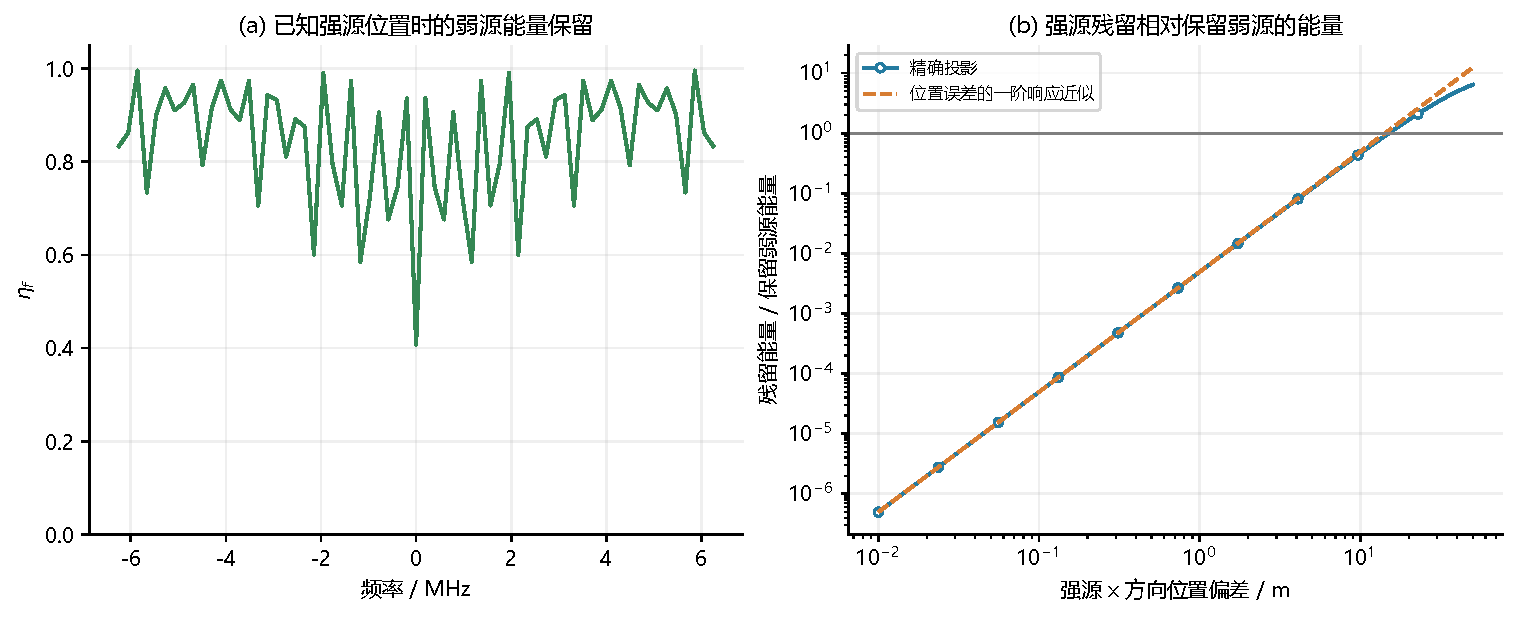
\includegraphics[width=.85\linewidth]{figures/fig_3_4.pdf}
\caption{投影机理的数值示例。}\label{fig:3.4}
\begin{minipage}{\linewidth}\small
采用本节所列频域参数。（a）各频点的弱源能量保留比例$\eta_m$；（b）强源沿$x$方向偏移0.01—50 m时，强源残留能量与准确投影后弱源能量之比，并比较式（\ref{eq:2.16}）的一阶响应近似。小偏差区间呈现近似二次增长。
\end{minipage}
\end{figure}

% Source block 151
小偏差区间内，强源残留与式（\ref{eq:2.16}）的二次能量近似相符。它解释了为什么强源误差虽小于定位成功阈值，仍可能影响弱源搜索；但没有给出实际求解中何时停止强源精修的判据。第\ref{sec:3.5}节的条件评分分析与这一误差传播关系相呼应。

% Source block 152
\subsection{成功率、处理时间与误差分布}\label{sec:3.8}

% Source block 153
\begin{figure}[H]
\centering
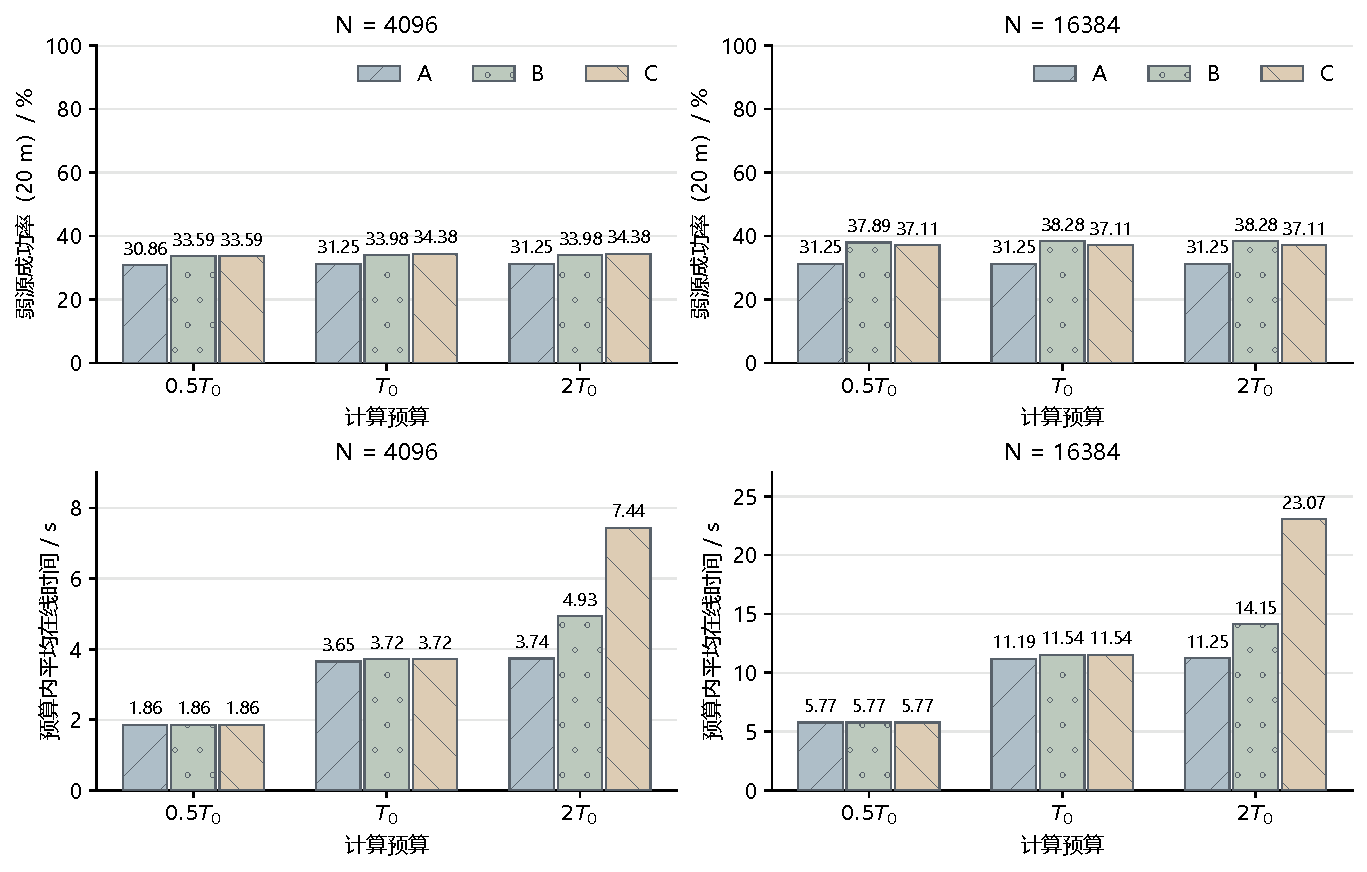
\includegraphics[width=.94\linewidth]{figures/fig_3_5.pdf}
\caption{三档预算下的弱源成功率与在线耗时。}\label{fig:3.5}
\begin{minipage}{\linewidth}\small
每种长度、每方法256条混合条件，横轴为$0.5T_0,T_0,2T_0$三档预算。上排为弱源20 m成功率；下排为计入该预算窗口的平均在线时间，提前完成时取实际耗时，否则取预算截止时间。评价采用截止前最近一次已完成的输出。表\ref{tab:3.8}另列整个运行窗口内的实测耗时。
\end{minipage}
\end{figure}

% Source block 156
\begin{table}[!htbp]
\centering
\caption{以$2T_0$为运行上限的实际平均耗时。}\label{tab:3.8}
\small
\setlength{\tabcolsep}{4pt}
\renewcommand{\arraystretch}{1.2}
\begin{tabularx}{\linewidth}{Y{1}Y{1}Y{1}Y{1}Y{1}}
\toprule
\textbf{长度} & \textbf{A / s} & \textbf{B / s} & \textbf{C / s} & \textbf{C/B} \\
\midrule
4096点 & 3.739 & 4.933 & 7.446 & 约1.51 \\
16384点 & 11.248 & 14.154 & 23.078 & 约1.63 \\
\bottomrule
\end{tabularx}
\end{table}

% Source block 158
C在507/512条混合任务中用尽$2T_0$窗口，相对B的耗时增加未带来成功率优势。三档预算下，各方法的弱源成功率变化很小，说明在当前配置中，仅延长同一搜索过程的运行时间并不足以改善候选覆盖。

% Source block 159
\begin{figure}[H]
\centering
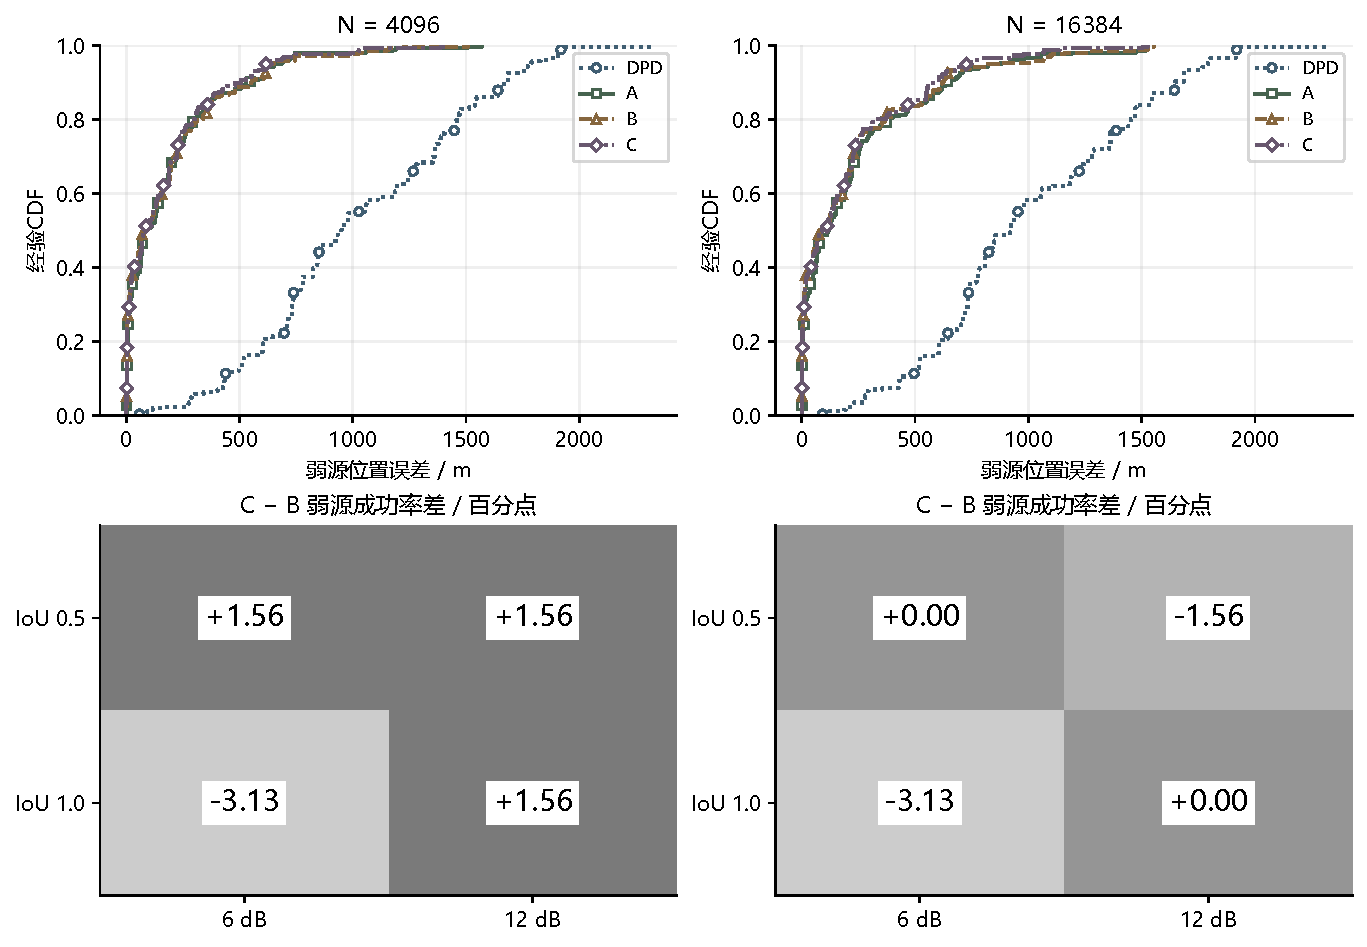
\includegraphics[width=.94\linewidth]{figures/fig_3_6.pdf}
\caption{未截断误差与条件分层。}\label{fig:3.6}
\begin{minipage}{\linewidth}\small
上排：各长度下的弱源平方距离最优匹配误差CDF，每曲线256条；下排：各长度、重叠和功率差条件下，C相对B的弱源20 m成功率差（单位：百分点），每格64条。误差横轴覆盖全部观测值。
\end{minipage}
\end{figure}

% Source block 162
图\ref{fig:3.6}显示，误差分布仍有明显长尾，C相对B的成功率变化依条件而异。RMSE较低与成功率提高并不等价，因而需结合成功率、未截断误差和处理时间评价搜索策略。

% Source block 163
\subsection{充分搜索的收益与代价}\label{sec:3.9}

根据第\ref{sec:3.6}节的诊断，固定方法D的5 m网格、前5个候选和更新轮数，在六个新布局上检查其作用。每个布局包含两种观测长度、两种频谱重叠和两档功率差，共$6\times2\times2\times2=48$个条件，每条件使用一组波形与噪声实现。完整方法B与D处理相同观测，均执行预定流程，不使用第一组实验的预算截止输出。

\begin{table}[!htbp]
\centering
\caption{六个新布局上的完整求解结果，成功半径20 m。}\label{tab:3.9}
\small
\setlength{\tabcolsep}{4pt}
\renewcommand{\arraystretch}{1.2}
\begin{tabularx}{\linewidth}{Y{0.55}Y{0.85}Y{0.85}Y{1.05}Y{1.05}Y{1.05}Y{1.05}Y{1.05}}
\toprule
方法 & \shortstack[l]{弱源\\成功数} & \shortstack[l]{双源\\成功数} & \shortstack[l]{强源\\成功数} & \shortstack[l]{GOSPA\\ / m} & \shortstack[l]{RMSE\\ / m} & \shortstack[l]{P95\\ / m} & \shortstack[l]{平均时间\\ / s} \\
\midrule
B & 8/48 & 8/48 & 48/48 & 69.16 & 128.56 & 343.98 & 8.04 \\
D & 40/48 & 40/48 & 48/48 & 18.37 & 64.28 & 121.40 & 31.10 \\
\bottomrule
\end{tabularx}
\end{table}

方法D恢复了B的32条弱源失败记录，并保留B原有的8条成功记录。弱源成功率由16.67\%升至83.33\%，总体RMSE由128.56 m降至64.28 m，但平均完整处理时间增至原来的3.87倍。该结果反映补充全局搜索与联合更新的合并作用，尚未分别量化两部分的收益。

\begin{figure}[H]
\centering
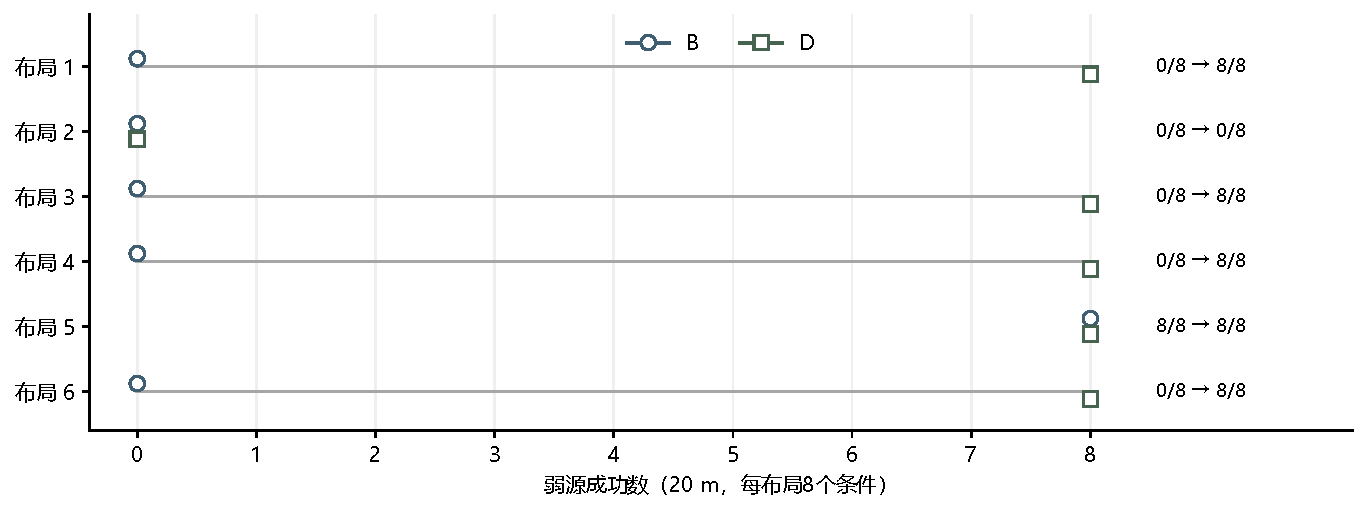
\includegraphics[width=.95\linewidth]{figures/fig_3_7.pdf}
\caption{六个新布局中方法B与D的弱源成功数。}\label{fig:3.7}
\begin{minipage}{\linewidth}\small
每布局8个条件，成功半径20 m；圆点为B，方点为D。位置重合的标记作少量纵向错位，横坐标保持真实成功数。布局编号仅用于本组比较。
\end{minipage}
\end{figure}

\begin{figure}[H]
\centering
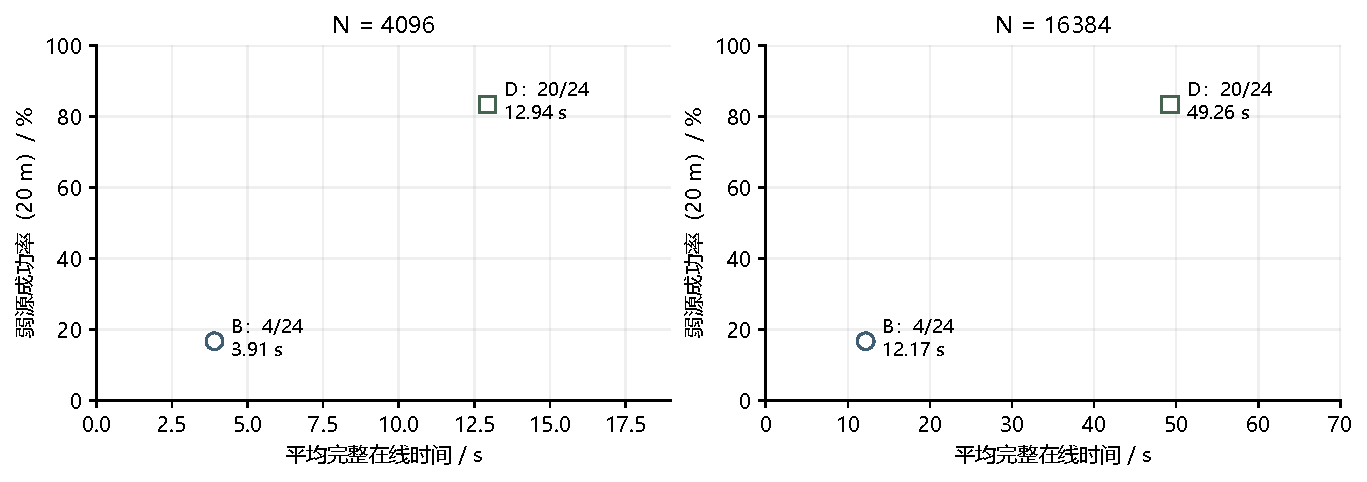
\includegraphics[width=.95\linewidth]{figures/fig_3_8.pdf}
\caption{两种观测长度下的成功率与完整处理时间。}\label{fig:3.8}
\begin{minipage}{\linewidth}\small
每种长度24个条件。4096点下，B与D的平均时间分别为3.91 s和12.94 s；16384点下分别为12.17 s和49.26 s。D的时间包含完整B及后续搜索，未按预算截断。
\end{minipage}
\end{figure}

两种长度下，方法D的弱源成功数均为20/24。剩余8条失败集中于布局2，弱源误差为83.72—290.93 m；该布局在两种长度、两种重叠和两档功率差下均未恢复。这种集中性表明失败与布局条件有关，但现有结果尚不能区分更细的候选遗漏、错误局部极值及位置耦合各自的作用。该组与前述32布局的样本不同，成功率和耗时均分别解释。

\subsection{固定样本上的区域细分比较}\label{sec:3.10}

为检验式（\ref{eq:cell-upper}）能否减少搜索量，在第\ref{sec:3.6}节的同一组24条诊断记录上比较四种单次弱源搜索策略：5 m均匀网格、横纵坐标各偏移5 m的10 m错位网格、得分优先细分和上界优先细分。各策略均固定原强源估计，保留前5个候选并采用相同的连续精修，保留评分不低于原估计的结果。这里的5 m扫描仅更新一次弱源位置，与逐源搜索并联合更新的完整方法D不同。

两种区域细分均从50 m网格开始，每个初始区域半边长为25 m，每次细分至多32个区域，网格评分上限为16384点，最小半边长为1.5625 m。得分优先细分按中心评分排序；上界优先细分按$U(\mathcal C)$排序，并在区域上界低于当前最佳评分时剪枝。与其对应的数值核验覆盖两种记录长度、零至两个固定源及四种区域尺度，共24组，未出现采样评分超过区域界的情况。这一核验检查数值实现的一致性，不用于评价搜索性能。

\begin{table}[!htbp]
\centering
\caption{固定强源估计下的单次弱源搜索比较。}\label{tab:region-search}
\small
\setlength{\tabcolsep}{4pt}
\renewcommand{\arraystretch}{1.2}
\begin{tabularx}{\linewidth}{Y{1.25}Y{0.95}Y{0.95}Y{1.15}Y{1.0}Y{0.7}}
\toprule
策略 & \shortstack[l]{历史失败组\\达标数} & \shortstack[l]{历史对照组\\达标数} & \shortstack[l]{平均网格\\评分点数} & \shortstack[l]{平均更新\\时间 / s} & \shortstack[l]{剪枝\\区域数} \\
\midrule
5 m均匀网格 & 15/16 & 8/8 & 160689.5 & 11.2231 & --- \\
10 m错位网格 & 14/16 & 8/8 & 39971.2 & 2.8870 & --- \\
得分优先细分 & 2/16 & 6/8 & 16384 & 1.2901 & --- \\
上界优先细分 & 9/16 & 6/8 & 16384 & 1.5700 & 0 \\
\bottomrule
\end{tabularx}
\par\smallskip
\begin{minipage}{\linewidth}\small
达标均指弱源误差不超过20 m。时间与评分点数按全部24条记录平均，时间包含候选精修，不包含先前的强源估计；网格评分点数不含连续优化中的函数评价。剪枝仅用于上界优先策略，该策略24条记录的剪枝数均为零。
\end{minipage}
\end{table}

在相同的16384点评分上限下，上界优先细分恢复9/16条历史失败，多于得分优先的2/16条，说明该上界有助于区域排序。但两者均用尽评分上限，且上界优先策略没有排除任何区域。其平均更新时间约为5 m扫描的14.0\%，恢复数却少6条，尚未达到相近的恢复能力。当前上界虽满足所采用响应模型下的约束，仍过于宽松，未实现有效剪枝。

10 m错位网格以5 m扫描约25.7\%的更新时间恢复14/16条历史失败，与第\ref{sec:3.6}节普通10 m扫描的恢复数相同。在两种网格结果不同的窄峰案例中，5 m扫描误差为0.805 m，错位10 m网格为48.54 m。错位采样可以改变候选位置，但该结果不足以说明其能够稳定替代加密网格。两种细分策略的历史对照达标数均为6/8，保留了原有6条20 m成功记录；5 m与错位10 m扫描还使另外2条对照达到20 m。

这组结果仅比较固定强源后的单次弱源更新，样本按历史失败与对照目的选取。相应恢复比例不能视为总体成功率，更新时间也不能直接解释为完整定位算法的加速比。

\subsection{阶段性结论}\label{sec:3.11}

% Source block 164
在32布局的比较中，逐源投影和联合更新将弱源20 m成功率提高至31\%—36\%，但仍低于孤立弱源的91\%—95\%。条件评分表明，大部分失败存在未被求解器找到的更优位置；部分记录的弱源评分还受到强源位置误差影响。

% Source block 165
响应变化量排序C相对普通区域搜索B未显示稳定收益。补充5 m全局搜索的方法D在六个新布局中将弱源成功数由8/48增至40/48，代价是平均完整处理时间增至3.87倍。在固定诊断样本上，区域上界改善了细分次序，但没有实现剪枝，恢复能力也低于加密网格。后续搜索设计需要同时减少无效评分和保留窄峰候选，仅延长运行时间或改变区域排序尚不足以解决这一问题。

% Source block 166
完整加密搜索后仍有一个布局的全部条件失败。固定强源的单次搜索比较不能解释这组剩余失败，仍需区分候选遗漏与位置耦合，并判断何时需要同时改变两个源的位置。

% Source block 168
\section{已知增益实验的讨论}\label{sec:4}

以下讨论对应附录\ref{sec:3}的既有搜索实验。正文第\ref{sec:new-results}节在新的信号与样本条件下比较了八种方法，第\ref{sec:new-discussion}节据此讨论后续问题。

% Source block 169
\subsection{窄峰宽度与搜索尺度}\label{sec:4.1}

% Source block 170
表\ref{tab:3.7}中，距真实位置4.523 m的格点评分低于远处错误峰，而真实位置附近的局部解误差为0.803 m。式（\ref{eq:2.17}）描述峰顶附近的二阶变化，但峰顶和曲率在搜索前都未知，尚不能直接据此确定网格间隔。

% Source block 171
式（\ref{eq:cell-upper}）已给出响应扰动下的区域评分上界，但现有比较中没有产生剪枝。当投影响应范数较小或区域内相位变化较大时，方向约束容易退化为残余能量上界。当前问题是如何利用中心评分、响应导数和残余收紧这一约束，同时控制计算代价。等效Fisher信息描述局部统计精度，评分Hessian描述单次观测的峰形；二者能否在可检验的条件下用于选择搜索尺度，仍需明确。

% Source block 172
\subsection{候选选择与计算分配}\label{sec:4.2}

% Source block 173
327条弱源失败中，292条在原强源估计下已有评分更高的真实位置。方法D在新布局上获得较多恢复，但平均耗时约为B的3.87倍。固定样本中的上界优先细分又弱于简单的错位网格，说明较复杂的区域规则未必能以相近计算量保留更多有效候选。需要判断中心评分较低时，哪些观测信息足以支持继续细分，以及少量补点评分、残余相关性或曲率估计能否减少全区域加密的开销。

% Source block 174
时延多假设可作为候选生成的一种选择。相对于参考站1，位置满足
% Source block 175
\begin{equation}\label{eq:4.1}
\Delta\tau_{\ell1}(\mathbf{p}) = \frac{\|\mathbf{p}-\mathbf{r}_\ell\|-\|\mathbf{p}-\mathbf{r}_1\|}{c}.
\end{equation}

% Source block 176
可以保留多个相关峰，以几何一致性生成位置候选，再用联合残差筛选\cite{ref01,ref02,ref03}。尚需讨论的是：在原始混合观测还是强源投影后的残余上提取时延更合适，何时施加跨站约束才能减少错误组合而不提前丢失弱源？这类方法的相关计算、假设组合和信号域验证均应计入耗时。

% Source block 177
同一组选例中，10 m网格将候选数从5增至32未增加恢复数，而5 m网格保留5个候选恢复了更多记录。因此，候选保留数与采样密度需要分别考虑。新的选择规则应保留均匀和错位网格作为参照，在相同连续优化配置下比较恢复能力与耗时，并在完整求解中核算总时间。

% Source block 178
\Needspace{.23\textheight}
\subsection{强源精度与联合位置更新}\label{sec:4.3}

% Source block 179
条件评分分析中，22条记录在替换真实强源位置后恢复了真弱源的评分优势，其中1条原强源误差小于20 m。式（\ref{eq:2.16}）给出小误差下的残留近似，但实际求解时真实误差未知，定位成功阈值也不能作为停止精修的依据。方法D剩余失败集中于同一布局，尚需判断逐源更新是否受到耦合局部解的限制。

% Source block 180
能否根据估计位置附近的曲率、响应导数和残余，判断继续精修强源与重新搜索弱源各自可能带来的改善？交替更新一次只改变一个位置，可能反复返回同一局部解；何时应保留多个强源位置假设，或联合更新四个位置坐标，仍需研究。四站系统中，扩大抑制子空间还会减少保留维数\cite{ref07}，因此比较这些做法时，需要同时考察强源残留、弱源信息损失和新增计算量。

% Source block 182
\clearpage
\end{document}
